\documentclass[12pt]{article}

% ------------------------------------------------------------------
% Shared preamble for the main manuscript (paper.tex) and the
% supplementary materials document (supplement.tex). Keeping this in
% one file ensures both documents typeset identically (fonts, float
% numbering macros, custom commands, etc.) even though they are
% compiled separately for submission.
% ------------------------------------------------------------------

% ------------------------------------------------------------------
% Encoding, fonts, and typography
% ------------------------------------------------------------------

\usepackage{iftex}
\ifPDFTeX
  \usepackage[T1]{fontenc}
  \usepackage[utf8]{inputenc}
  \usepackage{textcomp}
\else
  \usepackage{unicode-math}
  \defaultfontfeatures{Scale=MatchLowercase}
  \defaultfontfeatures[\rmfamily]{Ligatures=TeX,Scale=1}
\fi

\usepackage{lmodern}
\IfFileExists{upquote.sty}{\usepackage{upquote}}{}
\IfFileExists{microtype.sty}{%
  \usepackage{microtype}
  \UseMicrotypeSet[protrusion]{basicmath}
}{}

% ------------------------------------------------------------------
% Toggle: set to \includetitlepagetrue to include the separate title
% page (titlepage.tex) when compiling, e.g. for a blinded submission.
% ------------------------------------------------------------------
\newif\ifincludetitlepage
\includetitlepagefalse

% ------------------------------------------------------------------
% Page layout and paragraph formatting
% ------------------------------------------------------------------

\usepackage[
  lmargin=1in,
  rmargin=1in,
  tmargin=1in,
  bmargin=1in
]{geometry}

\usepackage{setspace}
\usepackage{parskip}
\setlength{\emergencystretch}{3em}

% ------------------------------------------------------------------
% Mathematics and color
% ------------------------------------------------------------------

\usepackage{amsmath}
\usepackage{xcolor}

% ------------------------------------------------------------------
% Tables
% ------------------------------------------------------------------

\usepackage{array}
\usepackage{booktabs}
\usepackage{multirow}
\usepackage{adjustbox}

\newcolumntype{L}{>{\raggedright\arraybackslash}p}
\newcolumntype{R}{>{\raggedleft\arraybackslash}p}
\newcolumntype{H}{%
  >{\raggedright\hangindent=0.5em\hangafter=1\arraybackslash}p
}

% ------------------------------------------------------------------
% Graphics, captions, and floats
% ------------------------------------------------------------------

\usepackage{graphicx}
\usepackage[labelfont=bf]{caption}
\usepackage{subcaption}
\usepackage{float}
\usepackage[section]{placeins}
\usepackage{afterpage}
\usepackage{pdflscape}

% ------------------------------------------------------------------
% Title and author formatting
% ------------------------------------------------------------------

\usepackage{titling}
\usepackage{authblk}

\setlength{\droptitle}{-2.2cm}
\posttitle{\par\end{center}\vskip 1.5em}
% \renewcommand\Authfont{\normalsize}
\renewcommand\Affilfont{\normalsize}

% ------------------------------------------------------------------
% Contents and section numbering
% ------------------------------------------------------------------

\usepackage{titletoc}
\setcounter{secnumdepth}{2}

% ------------------------------------------------------------------
% Pandoc/citeproc support
% ------------------------------------------------------------------

\NewDocumentCommand\citeproctext{}{}

\makeatletter
\let\@cite@ofmt\@firstofone
\def\@biblabel#1{}
\def\@cite#1#2{{#1\if@tempswa, #2\fi}}
\makeatother

\newlength{\cslhangindent}
\setlength{\cslhangindent}{1.5em}

\newenvironment{CSLReferences}[2]
  {\begin{list}{}{%
    \setlength{\itemindent}{0pt}
    \setlength{\leftmargin}{0pt}
    \setlength{\parsep}{0pt}
    \ifodd #1
      \setlength{\leftmargin}{\cslhangindent}
      \setlength{\itemindent}{-\cslhangindent}
    \fi
    \setlength{\itemsep}{#2\baselineskip}}}
  {\end{list}}

\providecommand{\tightlist}{%
  \setlength{\itemsep}{0pt}%
  \setlength{\parskip}{0pt}%
}

% ------------------------------------------------------------------
% Links and PDF metadata: load near the end
% ------------------------------------------------------------------

\usepackage[unicode]{hyperref}
\usepackage{bookmark}

\hypersetup{
  pdftitle={Attributes, Abstractions, and Combinations},
  pdfauthor={Hauke Licht; Leonce Röth},
  pdfkeywords={
    social groups,
    social attributes,
    computational text analysis,
    political behavior
  },
  colorlinks=true,
  linkcolor=black,
  citecolor=black,
  urlcolor=black,
  pdfcreator={LaTeX}
}

% ------------------------------------------------------------------
% Paper title, authors, and author affiliations
% ------------------------------------------------------------------


\title{%
    Attributes, Abstractions, and Combinations%
    \\\Large A New Taxonomy for Studying How Parties Invoke Social Groups%
}

\author[1]{%
  Hauke Licht%
  \thanks{%
    \href{mailto:Corresponding author: hauke.licht@uibk.ac.at}{Corresponding author: hauke.licht@uibk.ac.at}
  }
}
\author[2]{Leonce Röth}

\affil[1]{Department of Political Science \& Digital Science Center, University of Innsbruck, Austria}
\affil[2]{Geschwister Scholl Institute of Political Science, LMU Munich, Germany}
    
\date{September 14, 2026}


% ------------------------------------------------------------------
% Cross-referencing the main manuscript (paper.tex). The supplement
% contains a couple of \ref calls back into the main text (e.g.,
% Figure 5); xr-hyper resolves these via paper.aux. Build order
% matters -- see Makefile.
% ------------------------------------------------------------------
\usepackage{xr-hyper}
\externaldocument{paper}

\begin{document}

\clearpage
\appendix
\setcounter{page}{1}
\begin{center}
\Huge \scshape Supplemental Materials \par
\LARGE \bfseries Attributes, Abstractions, and Combinations \par
\medskip
\Large \normalfont Hauke Licht and Leonce Röth
\bigskip
\end{center}
\vfill
\renewcommand{\contentsname}{Contents}
\startcontents[appendix]
\printcontents[appendix]{}{1}{\setcounter{tocdepth}{2}}
\vfill
\clearpage

\counterwithin{figure}{section}
\counterwithin{table}{section}
\renewcommand\thefigure{\thesection\arabic{figure}}
\renewcommand\thetable{\thesection\arabic{table}}

\section{Dataset}\label{sec-apx_dataset}

We focus our application on social group references in the party manifestos of populist radical-right (PRR) and Green parties.
To this end, we compiled a corpus of party manifestos from 36 Western countries covering the period 1966--2021.
To enable comparisons with mainstream parties, we additionally include the manifestos of centre-left/social democratic and centre-right/conservative parties in four selected countries: Germany, Sweden, United Kingdom, and the United States.
Figure~\ref{figureA03} provides an overview of all covered cases.

Manifesto texts were obtained from secondary data sources, \emph{Manifesto Project Dataset} (Lehmann et al. 2023) and PoliDoc (Benoit et al. 2009).
Remaining gaps were filled through original data collection where possible.

In order to classify parties as being PRRPs, we follow the definition of Mudde (2007) and see nationalism as their core ideological feature.
For Green parties we follow Röth and Schwander (2021) or Dobson (2012) who define Green parties by a strong emphasis of ecologism and environmentalism and typically, but not always, incorporate the term ``Green'' in their party names.

In total, we processed 494 party manifestos (202 Green, 182 PRR, 56 Social Democratic, and 54 Conservative) into a corpus comprising 436,941 sentences.
Figure~\ref{figureA01} and Figure~\ref{figureA02} shows an overview of the number of manifestos and sentences by party family included in our corpus.

\begin{figure}[!th]
  \centering
  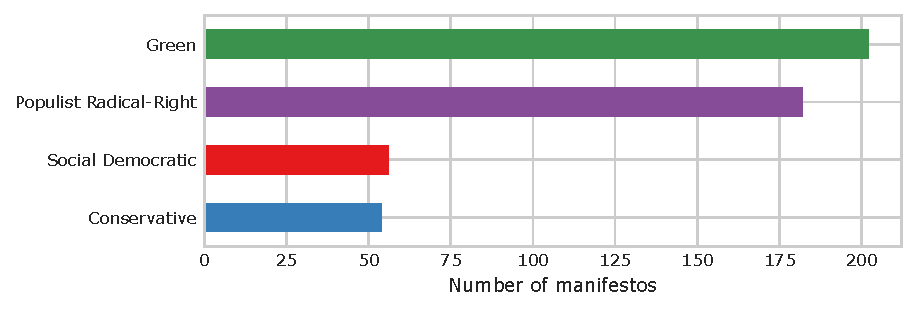
\includegraphics[keepaspectratio]{figures/figureA01.pdf}
  \caption{\label{figureA01}\protectNumber of manifestos by party family (all years).}
\end{figure}%

\begin{figure}[!th]
  \centering
  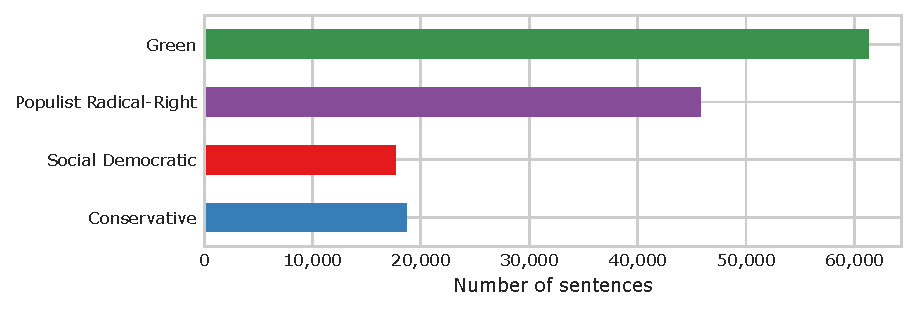
\includegraphics[keepaspectratio]{figures/figureA02.pdf}
  \caption{\label{figureA02}\protectNumber of sentences by party family (all years).}
\end{figure}%

\afterpage{
  \clearpage
  \thispagestyle{empty}
  \begin{figure}
    \centering
    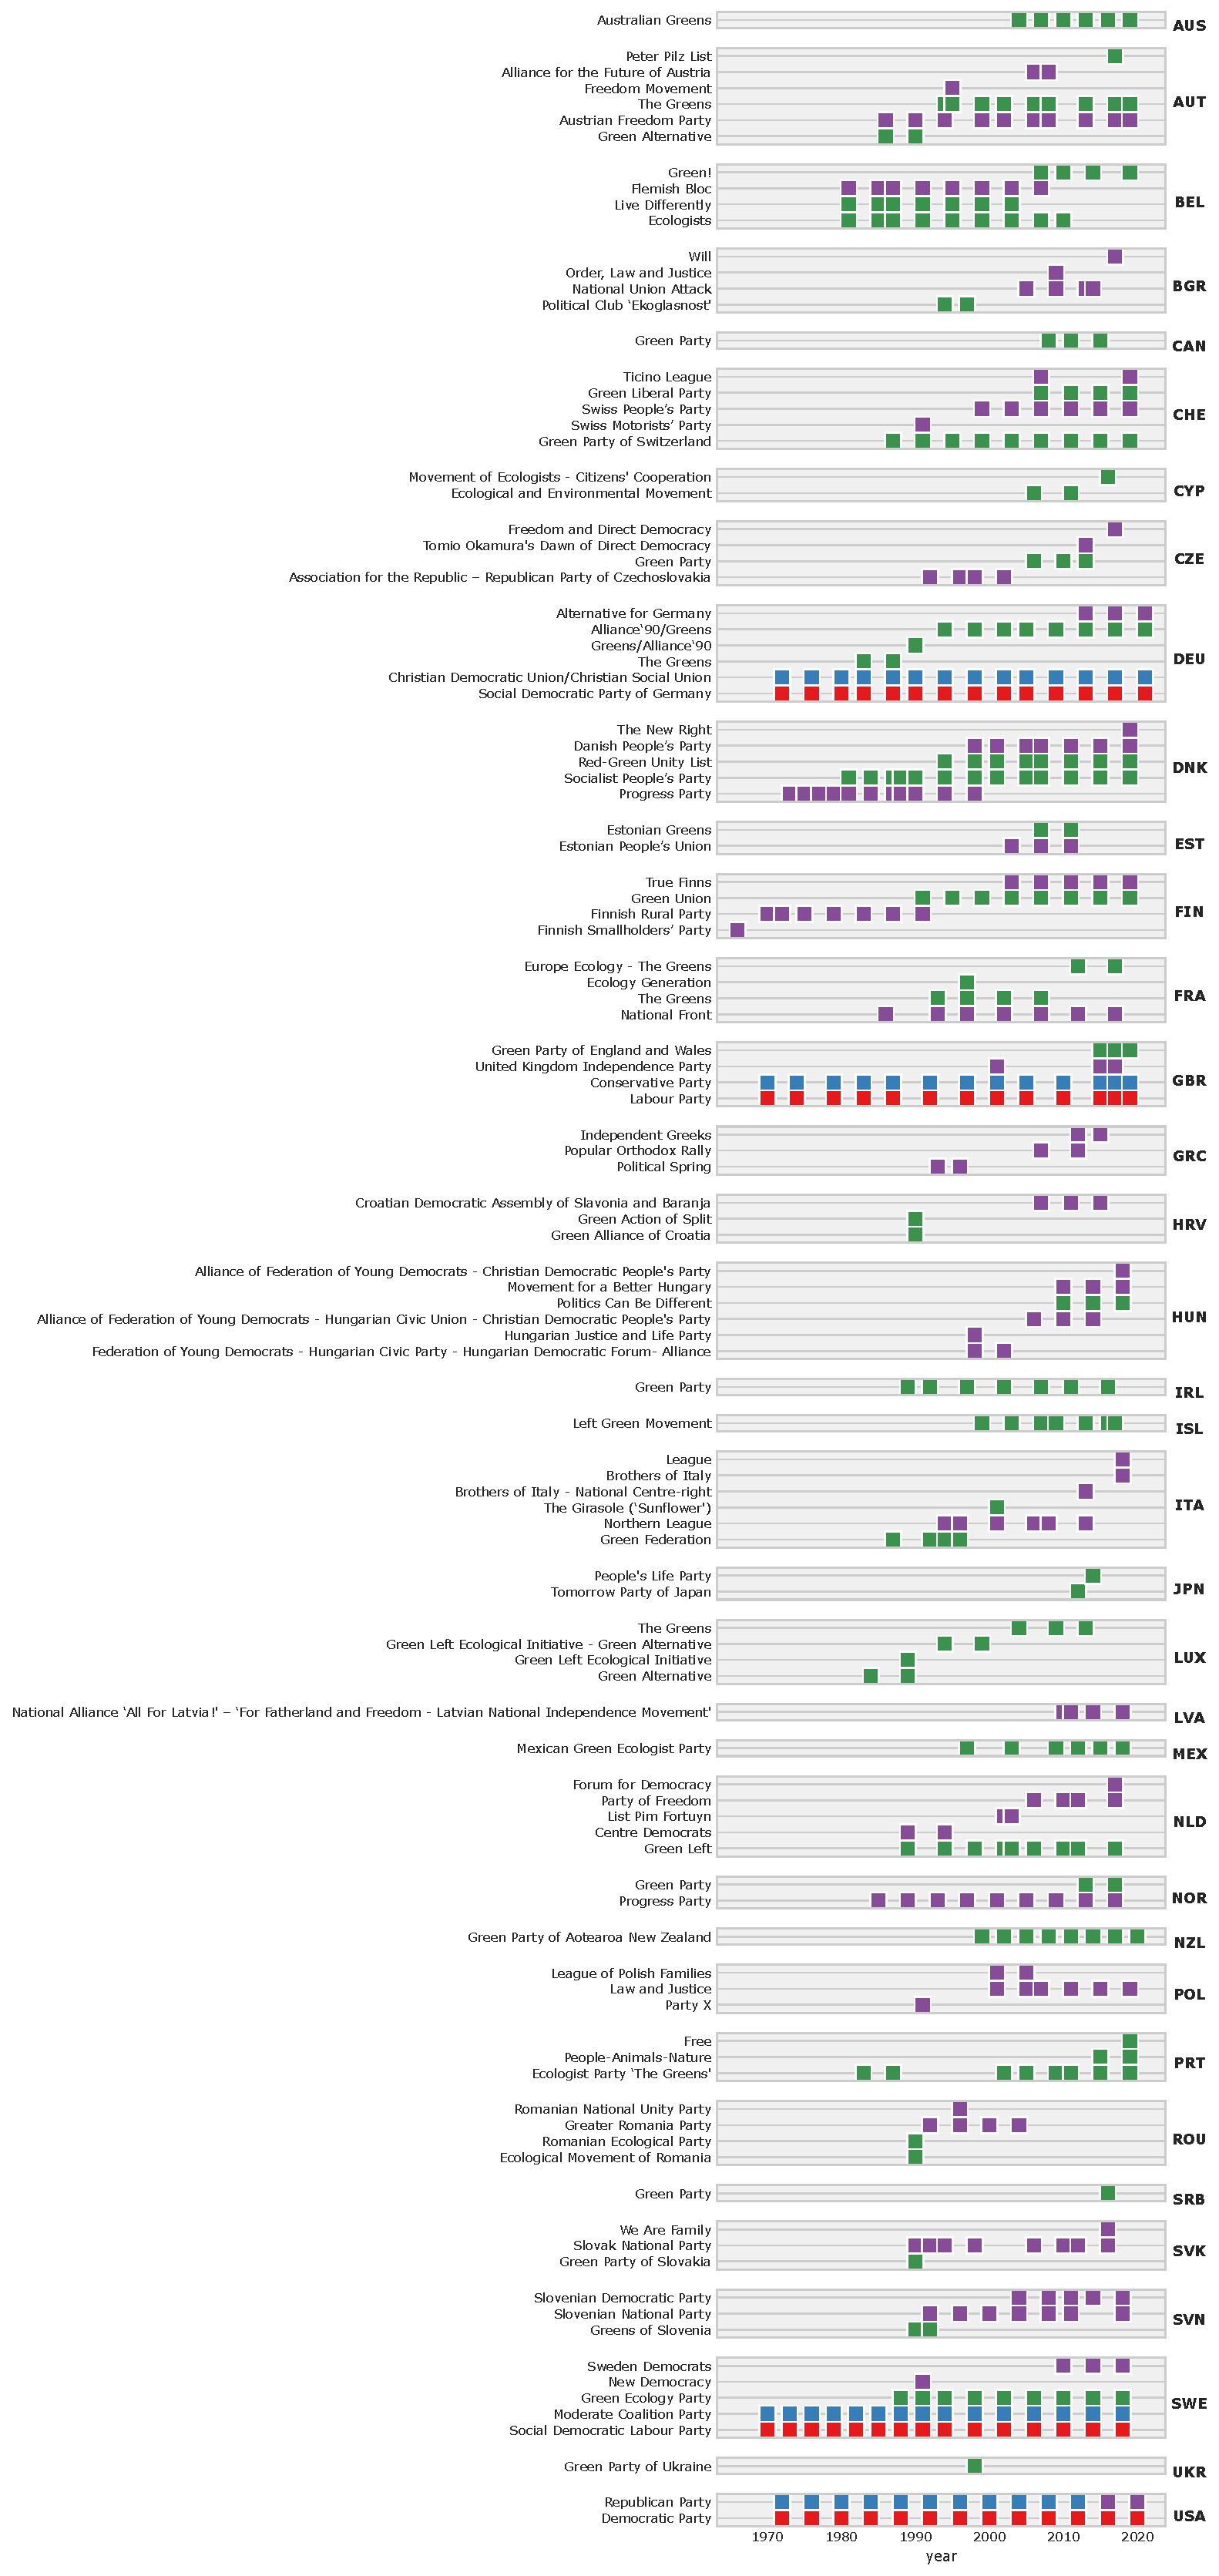
\includegraphics[keepaspectratio,height=0.92\textheight]{figures/figureA03.pdf}
    \caption{\label{figureA03}\protectOverview of cases included in our corpus. Each square represents a party in a given year, colored by its party family.}
  \end{figure}%
  \clearpage  
  
  \begin{figure}[!h]
    \centering
    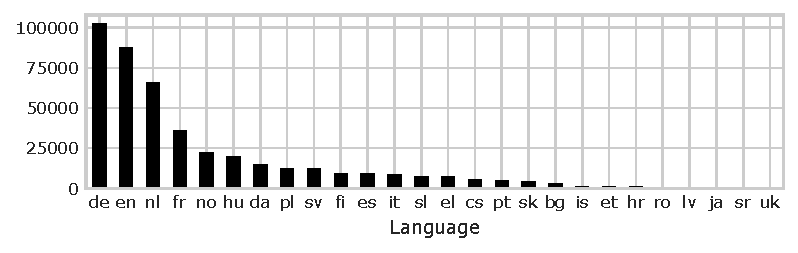
\includegraphics[keepaspectratio,width=\linewidth]{figures/figureA04.pdf}
    \caption{\label{figureA04}\protectLanguage coverage of the corpus of manifesto sentences. The corpus includes manifestos in 26 different languages. Languages denoted with their ISO 639-1 code. German (de), English (en), and Swedish (sv) are more strongly represented because our corpus also includes extensive time-series for social democratic and conservative parties in Germany, Sweden, the United Kingdom, and the United States. Other factors that contribute to languages' varying prevalence in our corpus are party system fragmentation and manifesto length, which, for example, explains the high number of Dutch (nl) sentences (many parties imply many manifestos).}
  \end{figure}%
  }
  
\clearpage


\section{Mention detection}\label{sec-apx_mention_detection}

Mention detection is the task of identifying which words or phrases in a sentence refer to social groups (Licht and Sczepanski 2025; Horne et al. 2025).
It is a prerequisite for classifying the attributes contained in social group mentions.

We produced the labeled data necessary for our application following the approach proposed by Licht and Sczepanski (2025), which combines sequence annotation (i.e., marking relevant phrases in sentences) and supervised token classification to extract any verbatim words or phrases used in a sentence to refer to social groups.

We proceeded in three annotation rounds, building on an active learning-like logic (cf. Miller et al. 2020) with the goal of maximizing the reliability and generalization of supervised classifiers trained on the collected annotations.
In the first round, we applied an informativeness-based sampling strategy (Kaufman 2024) to maximally diversify the selection of examples distributed for annotation, selecting 4315 sentences for annotation (stratifying by manifesto, i.e., party and election).
To manually annotate social group mentions in this sample, we recruited a research assistant (RA) that already had experience with this annotation task from prior projects and proved very reliable.\footnote{In addition to being qualified for the task through prior experience, they received detailed coding instructions explaining the concept of social group mentions with definitions and examples and we performed two rounds of training with the RA using 231 and 238 sentences, respectively, sampled from our target corpus.
  This allowed us to assert the coder's ability to identify social group mentions in the target data and provide them with feedback.
}.

To prepare the second annotation round, we used the RA's annotations from round one to train a preliminary token classifier, applied it to the remaining sentences in our corpus, and computed classification uncertainty for each sentence based on the predicted probabilities of the preliminary classifier.
We then sampled 2473 sentences (again, stratifying by manifesto) with high prediction uncertainty for annotation for the second round.
Importantly, this sampling strategy allowed us to progressively focus the human annotation effort on difficult cases.

We repeated this process one more time -- annotation, classifier training, uncertainty-based sampling -- to sample another 988 sentences for annotation in a third round.

\begin{figure}[!th]
  \centering
  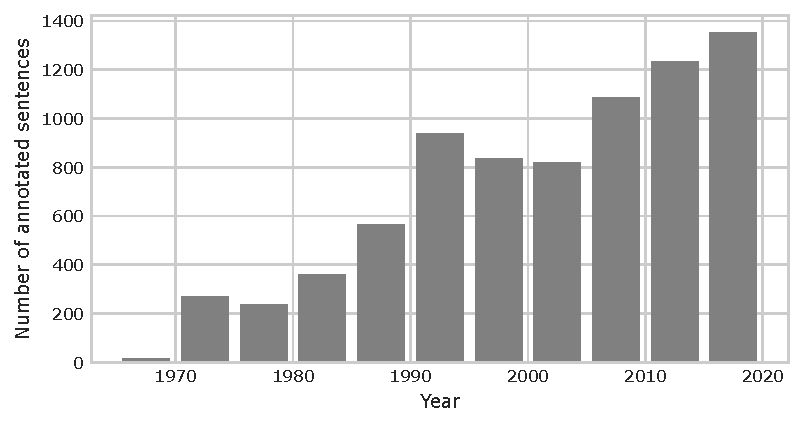
\includegraphics[keepaspectratio]{figures/figureB01.pdf}
  \caption{\label{figureB01}\protectDistribution of sentences annotated for group mention detection over time.}
\end{figure}%

Figure~\ref{figureB01} and Figure~\ref{figureB02} report the distributions of sentences we annotated for group mentions across years and countries, respectively.
Both distributions reflect the coverage and composition of our manifesto corpus (see Figure~\ref{figureA03}) and the fact that we stratified by manifesto, not country or time, when sampling in our three annotation rounds.
This means that more fragmented countries (e.g., Denmark) and/or countries with more elections are more strongly represented.
The alternative strategy of sampling equally across countries would, in contrast, have led to an underrepresentation of annotated examples from countries with many manifestos in our corpus.

Regarding the temporal distribution of our labeled sentences, it is notable that our data contains more sentences from manifestos from more recent decades.
This is because (a) Green and PRR parties only emerged gradually across the studied countries and (b) the missingness of manifesto raw texts tends to be comparatively higher in the 1970s and 1980s than in later decades.

Regarding the country distribution of annotated sentences, high-prevalence countries are those in which we have also covered a long time series of social democratic and conservative parties.
Moreover, Green and/or PRR parties existed for longer periods in some countries, so they feature more manifestos in our corpus and hence have higher overall sampling rates throughout our annotation rounds.

\begin{figure}[!th]
  \centering
  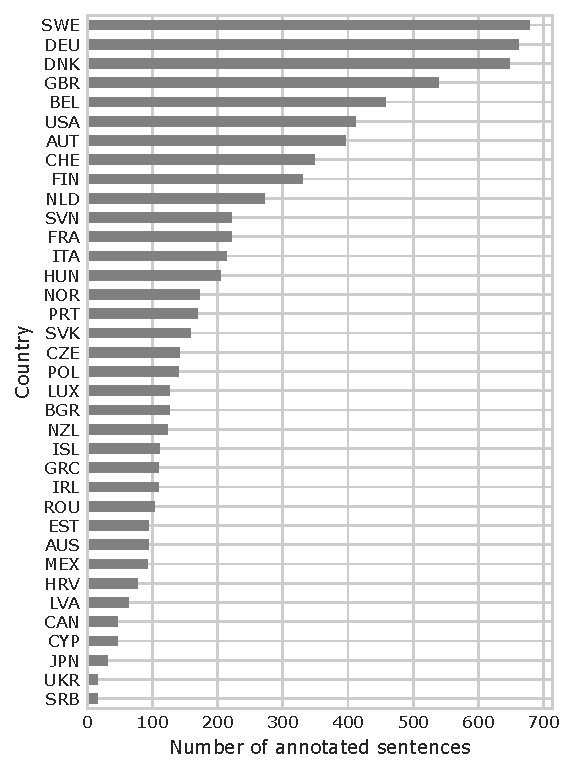
\includegraphics[keepaspectratio]{figures/figureB02.pdf}
  \caption{\label{figureB02}\protectDistribution of sentences annotated for group mention detection across countries.}
\end{figure}%


\clearpage

\section{Attribute classification}\label{sec-apx_attribute_classification}

\subsection{Coding instrument}\label{sec-coding_instrument}

Our coding instructions introduce the vertical/horizontal distinction, each of the attribute categories, as well as our ``universal'' group mention category, explain the available coding choices, and give examples.
Our coding instrument, implemented as a Qualtrics survey, presents annotators independently with one social group mention at a time (i.e., per page) in its respective sentence context, marking the mention in bold.

Below the display of the sentence, the annotator is first asked to indicate whether the highlighted mention is a ``universal'' mention per our definition.
If the annotator chose ``Yes'' for this coding dimension, our coding instructions asked them to proceed with the next instance on the next page.

If not, the annotator proceeds with coding the attribute categories for the vertical and horizontal attribute dimensions in turn.
For each of the dimensions, we tasked the annotator to indicate which of the respective attribute categories was contained in the highlighted social group mention, displaying the attribute categories below each other\footnote{We kept the categories' order fixed across examples to ease the cognitive load at annotation time.} in a multiple-choice grid with the answer options ``Yes'' or ``Unsure'' horizontally aligned.\footnote{We omitted options for ``No'' because not choosing ``Yes'' or ``Unsure'' for a given attribute category implied this coding choice.}
This procedure results in 17 annotations\footnote{1\(\times\) universal + 5\(\times\) vertical attributes + 11\(\times\) horizontal attributes} per mention-in-sentence-context instance and annotator.

\subsection{Annotation}\label{annotation-1}

In a first round of annotations, we have sampled 300 mentions-in-sentence-context examples from all sentences with at least one predicted social group mention, again using an informativeness-based sampling strategy.
Table~\ref{tableC01} reports the micro inter-annotator agreement (ICA) by attribute dimension from this round and indicates that our coders produced overall reliable annotations.
To resolve examples with disagreeing annotations, the author team reviewed any mention-in-sentence-context example with at least one disagreeing annotation to determine its final labels.

However, as expected, the prevalence of attribute categories in the labels collected in this first round turned out to be very imbalanced and we observed variation in ICA estimates across categories that could only partially be explained by low prevalence (see Table~\ref{tableC02}).
We therefore dedicated a second annotation round to collecting more annotations for difficult examples.
To this end, we fine-tuned a multilabel classifier to predict mentions-in-sentence-context examples' binary labels on the universal, vertical, horizontal indicators based on the consolidated annotations collected in the first round.
We applied this classifier to the mention-in-sentence-context instances not yet distributed for attribute annotation to obtain predicted probabilities.
We then computed classification uncertainty at the example level and selected the 150 most uncertain examples into a second annotation batch.

Table~\ref{tableC01} and Table~\ref{tableC02} show that, due to our focus on difficult examples, ICA was generally lower than in the first round.
We therefore used zero-shot in-context learning (Brown et al. 2020) to generate large language model (LLM) annotations for the examples in the second-round batch.
We then presented our annotators with the instances where the LLM disagreed with their judgment and tasked them to (independently) judge which annotation they viewed as more valid while blinding them to the source of the respective annotations.
The author team arbitrated the cases in which our annotators' independent judgments disagreed.
All instances from this second round were then consolidated into final labels and added to those of the first round.

\begin{table}[!th]
\centering
\caption{Inter-coder agreement estimates for attribute classifications computed at the level of attribute dimensions: universal, economic, and non-economic. Estimates are based on Krippendorff's $\alpha$ and the prevalence of `yes' annotations (prevalence) across all annotated examples in each annotation round.}
\label{tableC01}
\begin{tabular}{rrrrrrr}
\toprule
 & \multicolumn{3}{c}{Krippendorff's $\alpha$} & \multicolumn{3}{c}{prevalence} \\
annotation round & 1 & 2 & 3 & 1 & 2 & 3 \\
\midrule
universal & 0.697 & 0.259 & 0.000 & 0.275 & 0.144 & 0.006 \\
economic & 0.791 & 0.731 & 0.806 & 0.410 & 0.687 & 0.318 \\
non-economic & 0.754 & 0.474 & 0.752 & 0.563 & 0.727 & 0.844 \\
\bottomrule
\end{tabular}
\end{table}
%

\begin{table}[!th]
\centering
\caption{Inter-coder agreement estimates for attribute classifications computed at the level of economic and non-economic attribute categories. Estimates are based on Krippendorff's $\alpha$ and values in parentheses indicate the prevalence of `yes' annotations (prevalence) across all annotated examples in each annotation round.}
\label{tableC02}
\resizebox{\textwidth}{!}{%
\begin{tabular}{rrrrr}
\toprule
 & annotation round & 1 & 2 & 3 \\
dimension & category &  &  &  \\
\midrule
\multirow[t]{4}{*}{economic} & education & +0.799 (1.0\%) & +0.847 (8.0\%) & +0.888 (8.9\%) \\
 & employment status & +0.527 (8.8\%) & +0.607 (12.8\%) & +0.650 (6.7\%) \\
 & income/wealth/economic status & +0.694 (6.9\%) & +0.903 (13.0\%) & +0.745 (2.8\%) \\
 & occupation/profession & +0.804 (18.7\%) & +0.694 (28.8\%) & +0.241 (12.9\%) \\
\cmidrule(lr){1-5}
\multirow[t]{10}{*}{non-economic} & age & +0.832 (17.5\%) & +0.704 (12.8\%) & +0.442 (10.7\%) \\
 & crime & +0.659 (3.4\%) & +0.847 (8.0\%) & +0.842 (11.2\%) \\
 & ethnicity & +0.664 (1.3\%) & +0.658 (4.0\%) & +0.822 (25.1\%) \\
 & family & +0.765 (8.4\%) & +0.650 (6.7\%) & +0.753 (10.7\%) \\
 & gender/sexuality & +0.830 (2.4\%) & -0.021 (4.7\%) & +0.842 (25.8\%) \\
 & health & +0.906 (4.0\%) & +0.359 (10.7\%) & +0.607 (15.3\%) \\
 & nationality & +0.804 (12.9\%) & +0.581 (16.0\%) & +0.443 (20.8\%) \\
 & place/location & +0.662 (2.0\%) & +0.854 (2.7\%) & +0.496 (1.7\%) \\
 & religion & +0.666 (0.7\%) & +0.322 (3.3\%) & +0.959 (16.8\%) \\
 & shared values/mentalities &  & +0.567 (23.4\%) & +0.484 (5.0\%) \\
\bottomrule
\end{tabular}
}%
\end{table}
%

In a third round of annotation, we then addressed the problem of label class imbalance that clearly showed in the pooled set of multi-labeled mention-in-sentence-context instances from rounds one and two.
In particular, we focused on over-sampling likely examples of so far under-represented attribute categories in the vertical and horizontal attribute dimensions.
To identify likely examples for the given label categories, we used the attribute category definitions to define queries and used a pre-trained sentence embedding model to rank so far unannotated mention-in-sentence-context instances based on their cosine similarities to each of these queries.
To oversample likely examples of so far underrepresented categories, we defined quotas for each attribute category in inverse proportion to the categories' prevalence in the labeled instances from rounds one and two, using an annotation budget of 200 examples for round 3.
We then chose as many of the so far unannotated mention-in-sentence-context instances as the quota prescribed in descending order of their embeddings' similarities to the embedding of the respective attribute category definition query.
In total, this resulted in a sample of 180 mention-in-sentence-context examples for annotation in round 3.\footnote{Deviations from the annotation budget of 200 cases are explained by rounding in the computation of quotas and some mention-in-sentence-context instances that were ranked high for multiple attribute queries.}

Table~\ref{tableC01} shows that the attribute annotations of examples in this third round were overall highly reliable, which is likely explained by focusing on identifying \emph{likely} examples of each attribute category in this final round (in contrast to difficult instances in round 2).
Further, the consolidated labels from round 3 showed that our over-sampling strategy was effective as it helped to reduce the label class imbalance across the set of vertical and horizontal attribute categories.

A last round of annotation focused on conceptual consolidation and was performed by the authors.
Specifically, we manually reviewed any annotated examples that were labeled as combining certain attribute categories to determine whether the combination of these categories was conceptually valid and consistent with our attribute definitions.

\subsection{SetFit fine-tuning}\label{sec-apx_setfit}

Tunstall et al. (2022) propose a sentence transformer fine-tuning (SetFit) approach for few-shot learning in text classification applications.
In this framework, labeled examples in the training set are first used to construct pairs for contrastive embedding model fine-tuning.
This specializes a general-purpose sentence embedding model for representing social group mentions.
The contrastive finetuning task in the embedding finetuning step practically augments our 600 annotated examples to several thousand contrastive pairs, thus providing ample training material for embedding model finetuning.
This already effectively tunes the text representations that go into the attribute category multilabel classification head to our target concept.

Second, the fine-tuned embeddings are input to a classification head.
The classification head is the component that maps a mention's embedding into a multilabel attribute classification.
Both components are trained end-to-end for multilabel classification on labeled examples.

\subsubsection{Data splitting}\label{data-splitting}

We have first carefully split the 600 annotated examples into five training, validation and test folds to minimize leakage between the training and evaluation sets.
This is generally a crucial step in any supervised machine learning application, but it is particularly important in our application for several reasons.
First, simple random sampling does not account for the facts that
(a) mentions are embedded in sentences so that the same mention can appear in multiple sentences and
(b) some mentions are near duplicates of each other and having these in different splits can lead to overestimation of predictive performance.
Second, in the context of few-shot learning, it is particularly important to minimize leakage between the training and evaluation sets because the small number of training examples makes it more likely that a given example in the evaluation set is very similar to one in the training set, which can lead to overestimation of predictive performance.

\subsubsection{Evaluating implementation choices}\label{evaluating-implementation-choices}

We have thoroughly evaluated several implementation choices such as the base embedding model,\footnote{We evaluated models of varying size and architecture, including
  \href{https://huggingface.co/sentence-transformers/all-MiniLM-L6-v2}{\texttt{all-MiniLM-L6-v2}},
  \href{https://huggingface.co/sentence-transformers/all-mpnet-base-v2}{\texttt{all-mpnet-base-v2}},
  \href{https://huggingface.co/Alibaba-NLP/gte-modernbert-base}{\texttt{gte-modernbert-base}},
  \href{https://huggingface.co/nomic-ai/modernbert-embed-base}{\texttt{modernbert-embed-base}},
  \href{https://huggingface.co/ibm-granite/granite-embedding-english-r2}{\texttt{granite-embedding-english-r2}},
  \href{https://huggingface.co/google/embeddinggemma-300m}{\texttt{embeddinggemma-300m}},
  and
  \href{https://huggingface.co/Qwen/Qwen3-Embedding-0.6B}{\texttt{Qwen3-Embedding-0.6B}}} input formatting strategy,\footnote{We evaluated inputting only the group mention text, concatenating the mention text with its sentence context (pre- vs.~suffixing), and a custom span embedding strategy that pools the token embeddings of the mention text from the last layer of the embedding model.} and hyperparameter choices.

We have then used the training and validation split to examine the average performance of different base embedding models\footnote{We evaluated models of varying size and architecture, including
  \href{https://huggingface.co/sentence-transformers/all-MiniLM-L6-v2}{\texttt{all-MiniLM-L6-v2}},
  \href{https://huggingface.co/sentence-transformers/all-mpnet-base-v2}{\texttt{all-mpnet-base-v2}},
  \href{https://huggingface.co/Alibaba-NLP/gte-modernbert-base}{\texttt{gte-modernbert-base}},
  \href{https://huggingface.co/nomic-ai/modernbert-embed-base}{\texttt{modernbert-embed-base}},
  \href{https://huggingface.co/ibm-granite/granite-embedding-english-r2}{\texttt{granite-embedding-english-r2}},
  \href{https://huggingface.co/google/embeddinggemma-300m}{\texttt{embeddinggemma-300m}},
  and
  \href{https://huggingface.co/Qwen/Qwen3-Embedding-0.6B}{\texttt{Qwen3-Embedding-0.6B}}} and input formatting strategies\footnote{We evaluated inputting only the mention text, concatenating the mention text with its sentence context (pre- vs.~suffixing), and a custom span embedding strategy that pools the token embeddings of the mention text from the last layer of the embedding model.} and select the best-performing model and formatting strategy for each classifier.
Finally, we have trained the two classifiers on the full training set using the selected embedding model and input formatting strategy and evaluated their performance on the held-out test set.

\subsection{Validation}\label{sec-apx_validity}

\subsubsection{Content validity}\label{content-validity}

Besides their reliability, we also need to assess whether our classifiers categorize social group mentions in a substantively meaningful way.
We do so by analyzing the lexical patterns that characterize social group mentions assigned into our different attribute categories.
Specifically, we apply the ``fighting words'' bag-of-words method (Monroe et al. 2008) for identifying distinctive terms to quantify which terms are most strongly associated with our attribute categories.
 If our classifiers capture the attribute categories we conceptualize, their most distinctive terms should align with our substantive priors.

To enable this analysis, we have used our attribute classifiers to annotate all social group mentions extracted by our group mention detection model in our manifesto sentences corpus.
Note that we also include the manifestos of centre-left and -right parties covered by our case selection strategy in this validity assessment.

\paragraph{Universal group mentions}\label{universal-group-mentions}

\begin{figure}[!th]
  \centering
  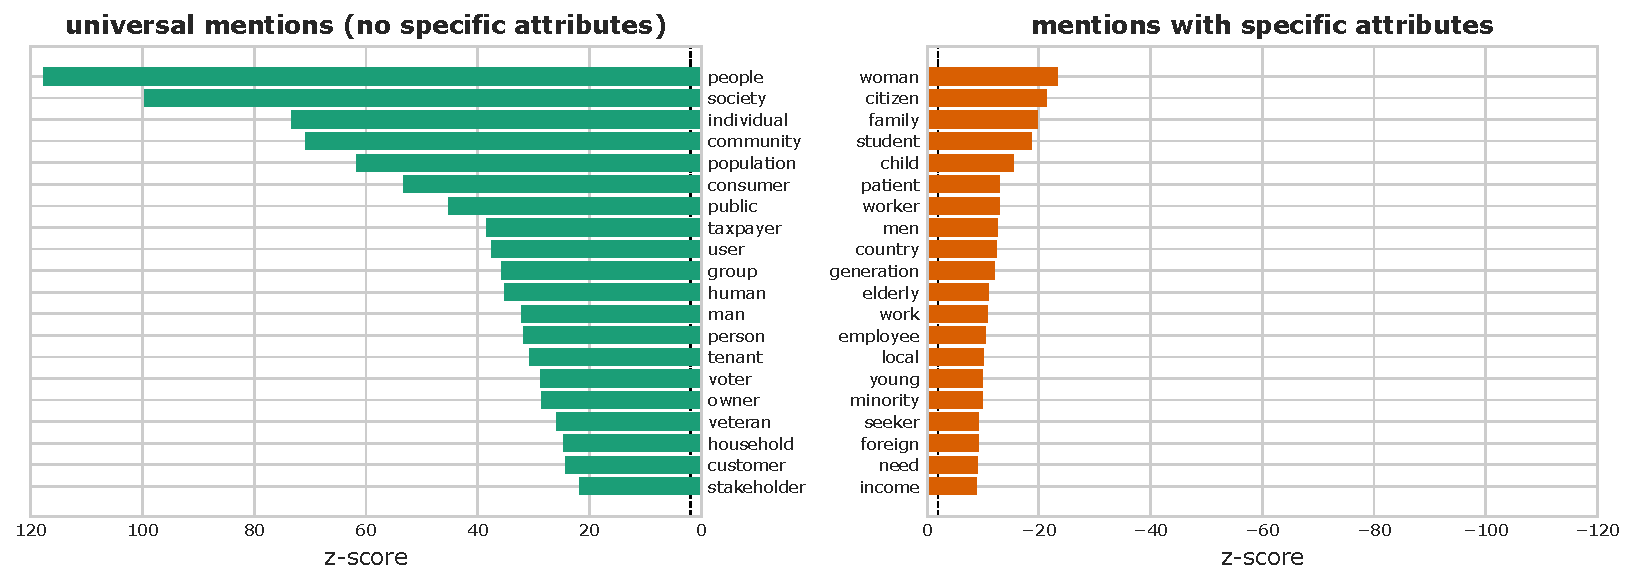
\includegraphics[keepaspectratio,width=\linewidth]{figures/figureC01.pdf}
  \caption{\label{figureC01}\protectMost distinctive words for mentions with no specific attributes (\emph{universal} mentions, left) vs. mentions with at least one economic or non-economic attribute (right).  Values plotted are $z$-scores from ``fighting words'' analysis.  Values above ±1.96 (vertical dashed line) can be considered significantly distinctive.}
\end{figure}%

We consider predicted group mentions that are predicted to contain no attributes as ``universal'' group references, that is, references to groups in general without specifying which kind of people they mean exactly.
To validate that the predicted absence of attributes in these mentions indeed reflects this conceptual category, we examine the most distinctive \(n\)-grams of these mentions by applying the ``fighting words'' method (Monroe et al. 2008) to all group mentions in our corpus, using a binary indicator of whether a mention is predicted to be a ``universal'' group reference as the grouping variable.\footnote{We have split mentions into tokens, removed English stop words, lemmatized tokens, computed uni-, bi-, and trigrams, and discarded any tokens that occurred in more than 80\% of mentions or in less than 5 mentions.}

Figure~\ref{figureC01} shows the top 20 most distinctive \(n\)-grams of ``universal'' group references.
The set of most distinctively ``universal'' terms includes tokens like ``people'', ``society'', ``everyone'', and similar terms that are used as generic collectivisms in the English language.
The most distinctively non-``universal'' terms, in turn, include denotational group labels like ``women'', ``students'', ``citizens'', and ``family''.

\paragraph{Attribute categories}\label{attribute-categories-1}

For the fighting words analysis of our attribute categories, we have first subset the dataset of extracted and labeled social group mentions to ``non-universal'' group mentions, that is, mentions that were classified as featuring at least one attribute covered by our taxonomy.
For each attribute category, we have then estimated the fighting words \(z\)-scores that measure distinctiveness by contrasting mentions that are predicted to feature the given attribute with those that are predicted to not feature it.

\afterpage{%
  \clearpage%
  \thispagestyle{empty}%
  \begin{landscape}%
  \begin{table}[!th]
\centering
\caption{Most distinctive terms for each attribute category, based on the ten tokens with the highest fighting words $z$-scores. The $z$-scores, reported in parentheses, indicate how strongly a term is associated with mentions in that attribute category compared to social group mentions that do feature attributes from this category. \emph{Note:} See \ref{figureC02} and \ref{figureC03} for visual presentations of the data.}
\label{tableC03}
\begin{tabular}{l L{4.5cm} L{0.85\textwidth}}
\toprule
 &  & top-10 most distinctiveterms \\
\midrule
\multirow[t]{4}{*}{economic} & education & student~(71.9), school~(47.4), education~(42.6), senior~(31.2), training~(25.0), pupil~(24.7), higher~(23.4), university~(23.1), study~(21.0), higher education~(19.8) \\
 & employment status & worker~(97.9), employee~(71.1), work~(49.7), working~(49.1), job~(35.0), workforce~(32.4), pensioner~(30.9), staff~(30.2), unemployed~(27.7), employed~(25.4) \\
 & income/wealth/economic status & need~(42.5), income~(35.8), group~(33.6), vulnerable~(32.4), low~(30.0), household~(29.6), class~(28.7), poor~(28.2), disadvantaged~(25.7), middle~(25.3) \\
 & occupation/profession & member~(39.1), public~(33.8), professional~(32.7), official~(26.5), representative~(26.0), personnel~(25.2), police~(23.8), politician~(23.2), health~(22.0), leader~(21.9) \\
\cmidrule(lr){1-3}
\multirow[t]{10}{*}{noneconomic} & age & child~(131.2), people~(59.0), young~(55.7), elderly~(36.7), future~(35.5), youth~(35.0), age~(34.6), generation~(34.5), year~(27.0), adult~(25.8) \\
 & crime & victim~(51.8), criminal~(47.6), violence~(30.0), drug~(28.2), prisoner~(28.1), crime~(27.5), prison~(23.6), sexual~(20.8), abuse~(20.7), terrorist~(20.5) \\
 & ethnicity & minority~(67.0), ethnic~(28.7), group~(26.3), black~(24.7), islander~(22.4), diverse~(20.3), national minority~(19.4), religious~(19.2), torres~(19.1), torres strait~(19.1) \\
 & family & child~(124.3), family~(71.4), parent~(31.6), single~(26.8), relative~(25.3), spouse~(24.5), caregiver~(20.9), couple~(18.1), mother~(17.7), family member~(16.4) \\
 & gender/sexuality & woman~(113.9), men~(72.5), couple~(27.6), girl~(27.2), sexual~(18.8), boy~(18.8), sex~(18.2), young woman~(15.5), mother~(15.1), position~(14.2) \\
 & health & person~(45.2), patient~(41.2), need~(39.2), people~(38.4), care~(34.6), vulnerable~(33.5), disabled~(30.7), affected~(27.2), sick~(25.7), special~(25.2) \\
 & nationality & citizen~(69.5), country~(42.8), american~(36.9), seeker~(30.5), nation~(26.6), national~(26.5), resident~(23.1), european~(22.9), foreign~(22.0), asylum~(21.4) \\
 & place/location & community~(58.7), local~(55.6), country~(49.9), resident~(44.8), rural~(35.4), living~(35.1), population~(29.4), germany~(28.0), area~(27.3), inhabitant~(26.5) \\
 & religion & community~(26.4), religious~(26.3), ethnic~(25.5), minority~(22.9), christian~(19.9), muslim~(19.2), faith~(18.8), multicultural~(17.6), different~(17.0), islamic~(16.9) \\
 & shared values/mentalities & society~(98.1), want~(38.3), free~(27.4), right~(27.2), life~(23.8), civil~(22.0), human~(20.9), democratic~(20.8), value~(19.5), green~(19.0) \\
\bottomrule
\end{tabular}
\end{table}
%
  \end{landscape}%
  %\clearpage%
}%

Table~\ref{tableC03} reports the top-10 tokens for each attribute category in our taxonomy resulting from this analysis.
Overall, the most distinctive terms strongly align with our expectations of the valid content of these categories.
For example, the most distinctive tokens for the economic attribute category \emph{education} are a semantically highly coherent cluster of terms related to groups (``students'' and ``pupils'') and contexts related to education (``school'', ``university'', and ``training'').
And for our novel \emph{shared values/mentalities} category, the most distinctive tokens feature many value-based adjectives and the lemmas of ``society'', which stands out because value-based group references tend to center on parties' visions of a society with certain shared values.
We view these results as strong evidence of the content validity of our classifiers.

\begin{figure}[!th]
  \centering
  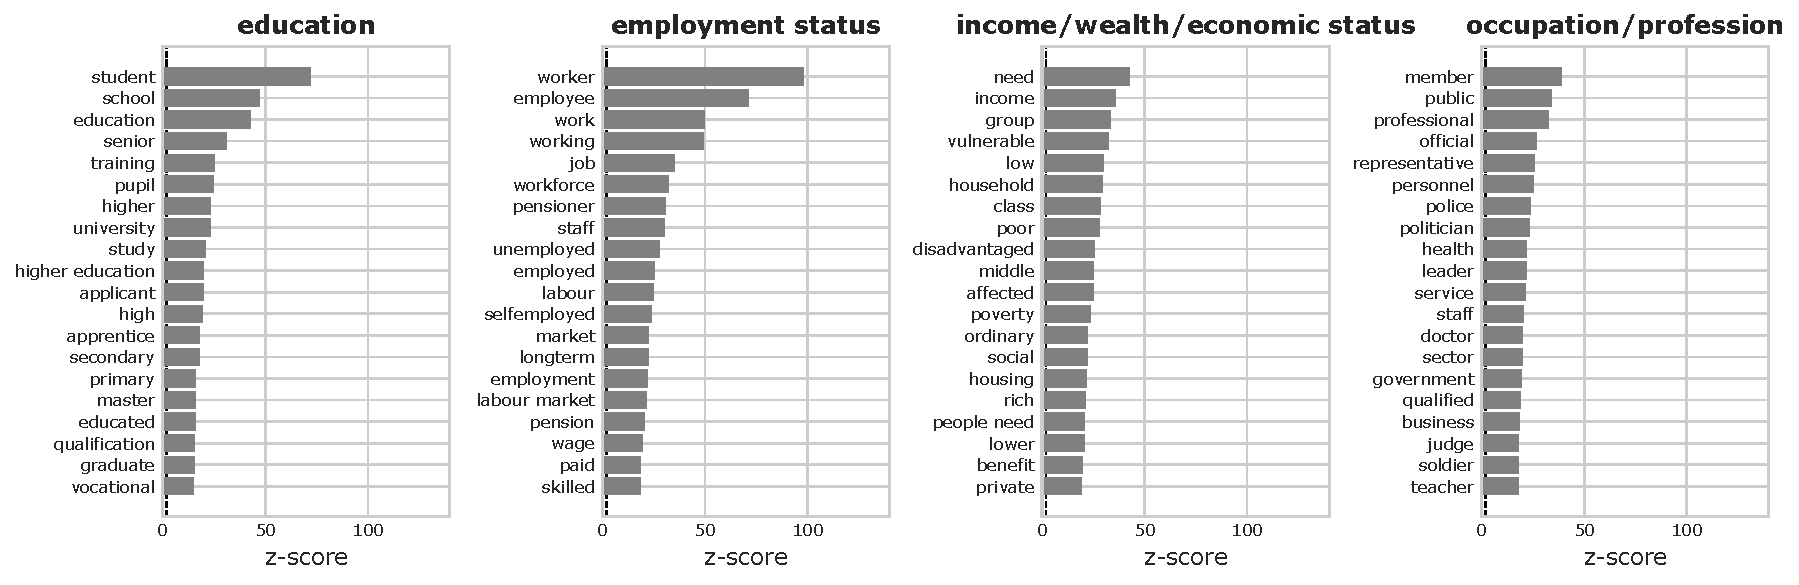
\includegraphics[keepaspectratio,width=\linewidth]{figures/figureC02.pdf}
  \caption{\label{figureC02}\protectMost distinctive words of social group mentions categorized as featuring a specific economic attribute. Values plotted are $z$-scores from ``fighting words'' analysis computed for mentions in focal category vs. all other non-universal mentions. Values above ±1.96 (vertical dashed line) can be considered significantly distinctive.}
\end{figure}%

\begin{figure}[!th]
  \centering
  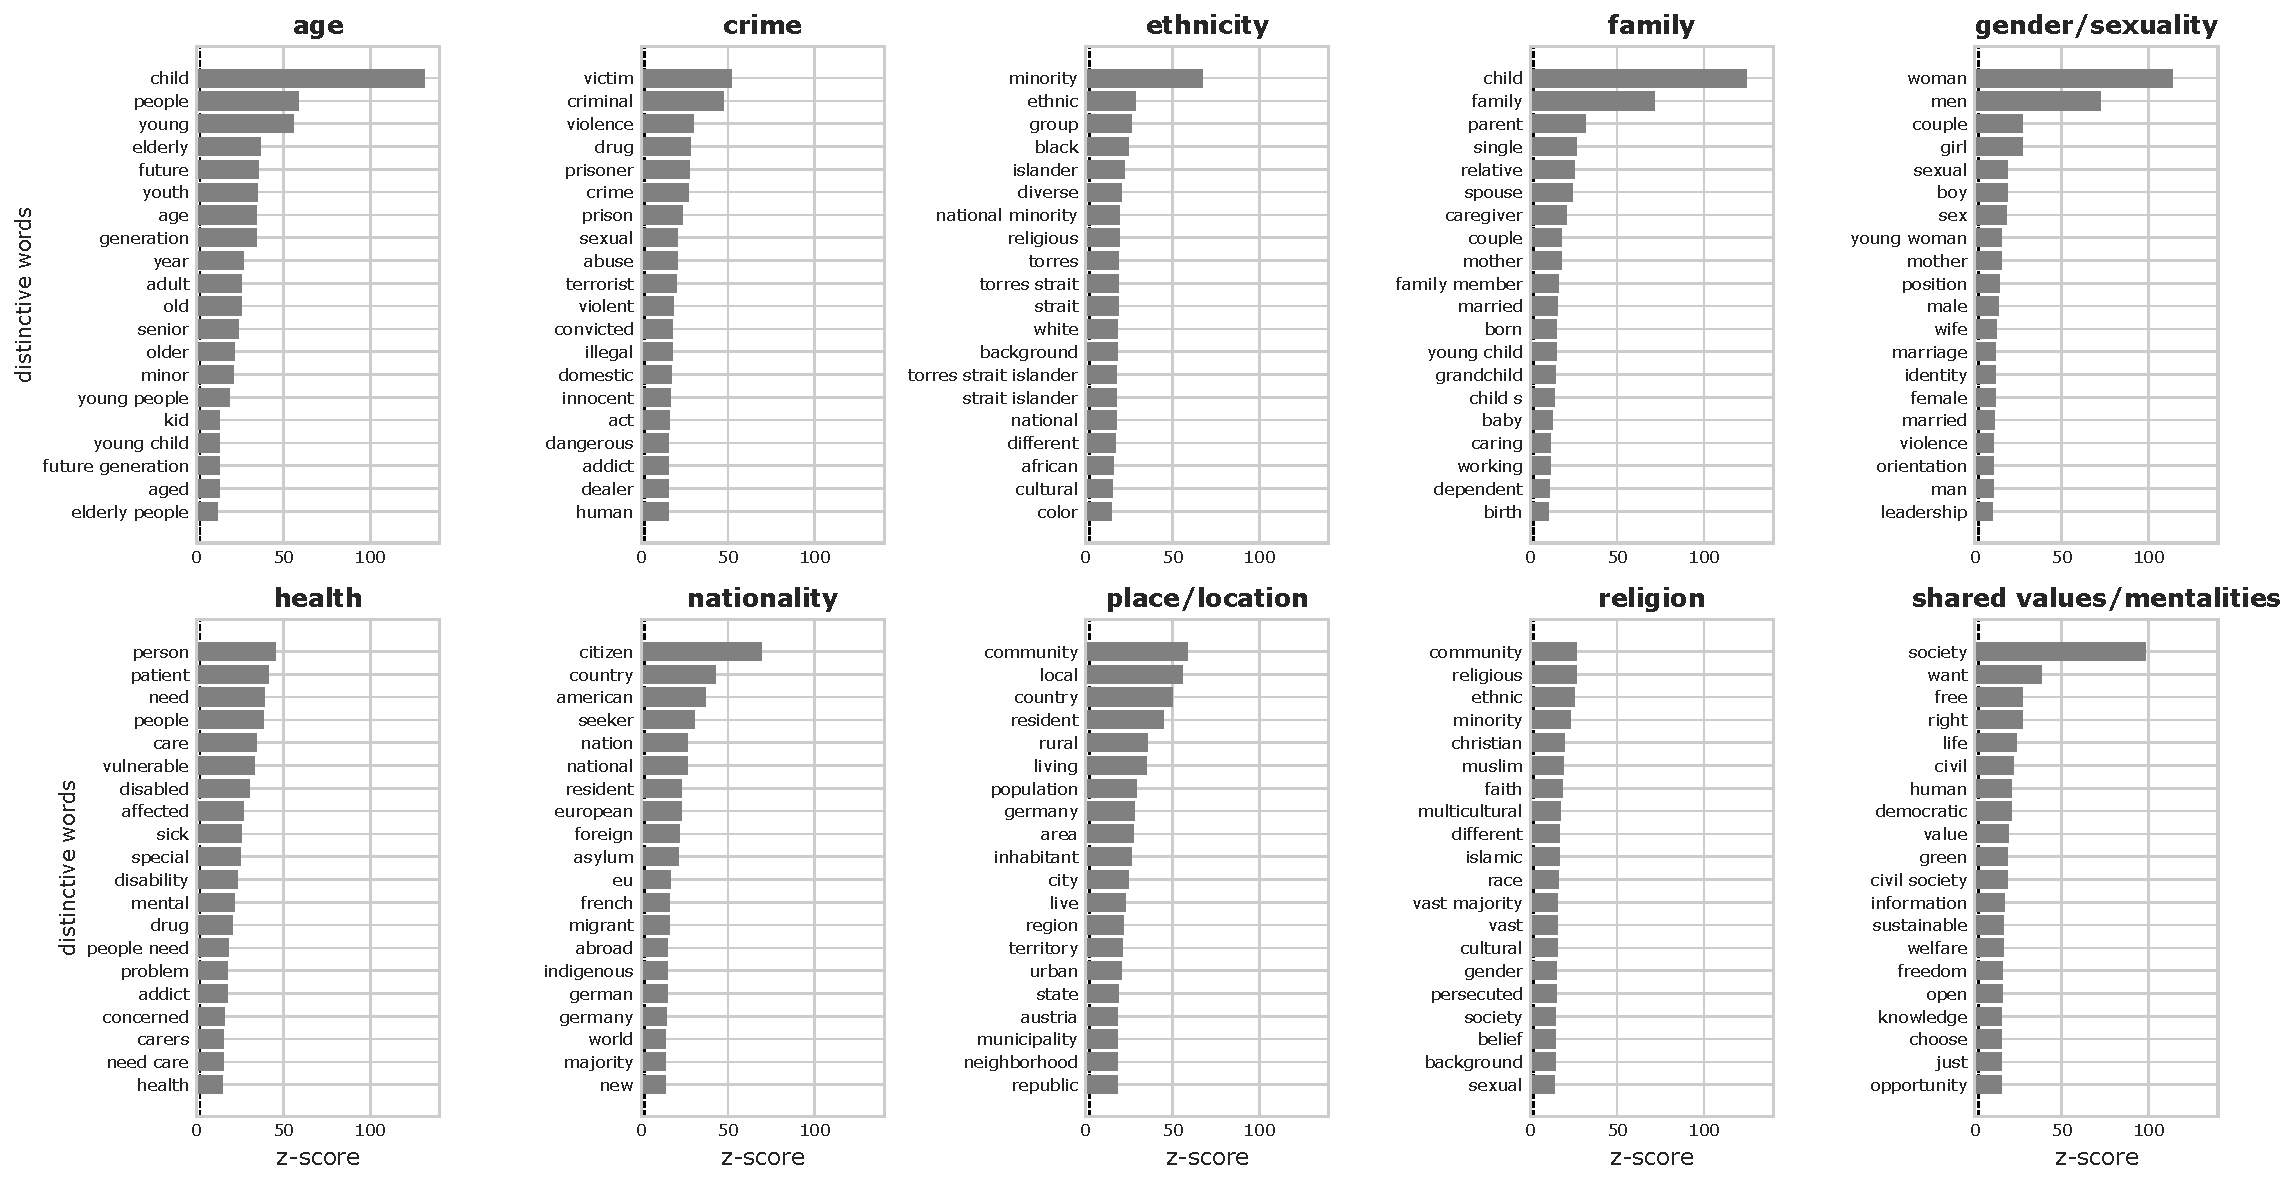
\includegraphics[keepaspectratio,width=\linewidth]{figures/figureC03.pdf}
  \caption{\label{figureC03}\protectMost distinctive words for social group mentions categorized as featuring a specific non-economic attribute. Values plotted are $z$-scores from ``fighting words'' analysis computed for mentions in focal category vs. all other non-universal mentions. Values above ±1.96 (vertical dashed line) can be considered significantly distinctive.}
\end{figure}%

The clarity of the top terms raises the question of whether the mention-level attribute classification could also be achieved with a set of rather simple dictionaries.
Additional analyses reported in Table~\ref{tableC04} speak against this simple alternative for most attribute categories.
While in the case of attribute categories like \emph{family}, \emph{age}, \emph{employment status} or \emph{education}, between 88\% and 70\% of mentions classified as featuring an attribute of the respective category also contain one of the top-10 terms of this category shown in Table~\ref{tableC03}, this estimate of recall of the top-10 terms is much lower for categories like \emph{religion} (42\%), \emph{nationality} (36\%), \emph{income/wealth/economic status} (33\%) or \emph{occupation/profession} (20\%).\footnote{Increasing the number of top terms to 40 or 50 only mitigates this partially with diminishing returns.} The latter group of categories thus seem to be centered on clear semantic clusters; our classifiers are able to capture them relatively reliably but the small sets of most-distinctive lexical features are not.
This conjuncture is supported by the qualitative insights we gained during annotations as well as the overall lower magnitude of the \(z\)-scores for these categories.
In sum, while indicating the high content validity of our classifiers, the most distinctive terms alone do not fully capture the essence of mentions in the respective attribute categories.

\begin{table}[!th]
\centering
\caption{Performance of the top $k$ terms for each attribute category in predicting the presence of that attribute in mentions. The table reports the proportion of mentions in each attribute category that contain at least one of the top $k$ terms for that category. The top $k$ terms are determined based on the ten tokens with the highest fighting words $z$-scores.}
\label{tableC04}
\begin{tabular}{rrrrrrr}
\toprule
 &  & \multicolumn{5}{c}{top $k$ terms} \\
 &  & 10 & 20 & 30 & 40 & 50 \\
\midrule
\multirow[t]{4}{*}{economic} & employment status & 0.793 & 0.830 & 0.852 & 0.878 & 0.889 \\
 & education & 0.701 & 0.780 & 0.817 & 0.837 & 0.849 \\
 & income/wealth/economic status & 0.329 & 0.446 & 0.527 & 0.585 & 0.613 \\
 & occupation/profession & 0.200 & 0.362 & 0.412 & 0.464 & 0.534 \\
\cmidrule(lr){1-7}
\multirow[t]{10}{*}{noneconomic} & family & 0.883 & 0.894 & 0.910 & 0.916 & 0.918 \\
 & age & 0.843 & 0.888 & 0.895 & 0.905 & 0.910 \\
 & gender/sexuality & 0.809 & 0.837 & 0.850 & 0.871 & 0.872 \\
 & health & 0.742 & 0.848 & 0.877 & 0.895 & 0.903 \\
 & ethnicity & 0.609 & 0.690 & 0.768 & 0.803 & 0.810 \\
 & place/location & 0.538 & 0.622 & 0.666 & 0.678 & 0.684 \\
 & shared values/mentalities & 0.486 & 0.512 & 0.555 & 0.592 & 0.620 \\
 & crime & 0.476 & 0.539 & 0.683 & 0.713 & 0.733 \\
 & religion & 0.420 & 0.501 & 0.533 & 0.538 & 0.542 \\
 & nationality & 0.367 & 0.411 & 0.421 & 0.507 & 0.513 \\
\bottomrule
\end{tabular}
\end{table}
%

\clearpage

\subsubsection{Comparison to other categorization schemes}\label{sec-convergence}

To further validate our attribute-centered social group mention classification approach, we compare the classifications produced with our scheme and classifiers with those produced by two existing \emph{group} categorization schemes developed by Thau (2019) and Horne et al. (2025), respectively.
This analysis shows both alignment and key differences between the schemes, highlighting the added analytical value of our attribute-centered approach, that takes attribute combinations and varying levels of abstraction into account.

\paragraph{Comparison to Thau's social group category classifications}\label{sec-thau_crossvalidation}

Thau (2019) has the analytical goal in common with our study.
He focuses on identifying \emph{and} classifying group mentions in the party manifestos of the British \emph{Labour} and \emph{Conservative} parties (1964-2015; cf. Thau (2021)) -- cases also covered by our corpus and samples of human-annotated texts.
He has developed a group categorization scheme that differentiates between five group types, including the types \emph{Social group} and \emph{Professional group}.
Within \emph{Social group} mentions, he further distinguishes between nine group categories.

However, a critical distinction between Thau's and our approach is that he assigns each group mention that his annotators identified to one and only one social group category.
In contrast, our taxonomy and classifiers account for the logic of attribute combination by allowing each mention to be assigned to multiple attribute categories.
This overlap in case coverage and analytical goal but difference in measurement strategy allows us to directly clarify the added value of multi-label attribute classification of our approach.

To compare our approach to Thau's group category annotations, we have applied our classifiers to the 4,018 human-labeled social and professional group mention examples in his annotated data.\footnote{Our corpus and samples of human-annotated texts also include \emph{Labour} and \emph{Conservative} party manifestos, making this an in-sample analysis.}
This allows us to analyze how our attribute-centered classification aligns with his group categories.
It also enables us to analyze how often our different attribute categories have been assigned to group mentions grouped into one group category in Thau's scheme, thus offering insights into what might have been lost in annotation by forcing single-class assignments.

\begin{figure}[!th]
  \centering
  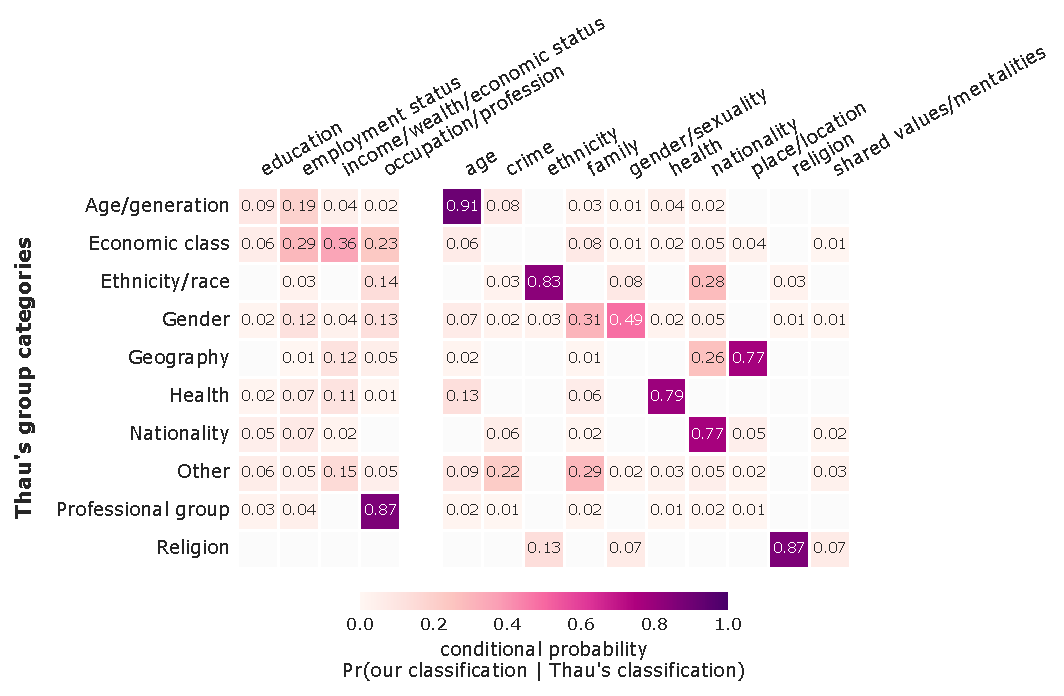
\includegraphics[keepaspectratio,width=\linewidth]{figures/figureC04.pdf}
  \caption{\label{figureC04}\protectCorrespondence of Thau's social group categorizations with our group attribute classifications. Numbers report the probability that a mention assigned by Thau's coders to one of his social group categories (shown on y-axis) has been labeled as featuring a given social attribute in our classification scheme (shown on x-axis). \emph{Note:} Values below 0.009 not plotted to ease readability.}
\end{figure}%

Figure~\ref{figureC04} shows the results of this analysis by reporting the probability that our classifiers label a mention with an attribute (x-axis), given the mentions' categorization in Thau's data (y-axis).
On the one hand, this shows strong correspondence between some of Thau's group categories and our attribute categories.
For example, 91\% of Thau's \emph{Age/generation} mentions are labeled as \emph{age} by our classifier, 83\% of mentions in his \emph{Ethnicity/race} category are labeled as \emph{ethnicity} by our classifier, and 87\% of group mentions in his \emph{Professional group} category are also classified as featuring an \emph{occupation/profession}-related attribute by our classifiers.

However, Figure~\ref{figureC04} also shows diversity within the mentions that Thau's annotators have assigned to only one of the group categories in his schemes.
For example, while 91\% of Thau's \emph{Age/generation} mentions are labeled as \emph{age} by our classifier, many of them are (also) classified as \emph{employment status} (19\%) and/or \emph{education} (10\%).
Categories like \emph{Economic class} or \emph{Gender} show particularly diverse attribute patterns, with mentions linked to several attributes (e.g., \emph{employment status}, \emph{income/wealth/economic status}, \emph{occupation/profession}).
These cases highlight the strength of the varying levels of abstraction in our taxonomy: they add analytical value by breaking down broad categories into specific attributes, allowing more detailed analysis of social class and status communication.

\begin{table}[!th]
\centering
\caption{Examples of verbatim group mentions with conflicting group category annotations in data by Thau (2019) for category combinations that were confused more than 10 times. Each row shows (at most) three examples of verbatim group mentions that have been categorized into one of the following categories in different sentence contexts in the corpus and thus have \"conflicting\" labels. $N$ reports the total number of mentions that exhibit the shown category confusion (in all 3,571 mentions).}
\label{tableC05}
\begin{tabular}{p{2.2in} l L{3in}}
\toprule
attribute combination & $N$ & examples \\
\midrule
Age/generation + Economic class & 50 & ``homeless 16 and 17 year olds''; ``young people in full-time higher education''; ``the young unemployed'' \\
Age/generation + Other & 29 & ``young users of hard drugs''; ``secondary age pupils''; ``persistent juvenile offenders'' \\
Economic class + Gender & 23 & ``women at work''; ``men who work in the public services''; ``Women at work'' \\
Economic class + Geography & 43 & ``the richest and poorest areas in our country''; ``rural businesses''; ``small local firms'' \\
Economic class + Nationality & 11 & ``migrant workers''; ``People coming to Britain from the EU for work''; ``skilled foreign workers'' \\
Economic class + Other & 94 & ``low income families''; ``families where all parents are working''; ``pensioner couples'' \\
Geography + Other & 13 & ``the community''; ``pupils in less advantaged areas''; ``community'' \\
\bottomrule
\end{tabular}
\end{table}
%

In particular, our comparison to Thau's human-annotated social group categorization data underscores the added value of taking attribute combination into account in group mention labeling.
The idea of \textbf{attribute combination} is that social group mentions often involve multiple social attributes at the same time and that from a methodological point of view, this requires multi-label classification.
Thau's coding scheme, however, is single-label, meaning that each group mention is assigned to one and only one group category.

Table~\ref{tableC05} illustrates the consequence of this annotation design choice by giving examples from Thau's data where the same verbatim group mentions were categorized into different group categories in his scheme at different times of the annotation process.
For example, the group mention ``homeless 16 and 17 year olds'' has been classified as both \emph{Economic class} and \emph{Age/generation} in this data, and this label confusion occurred for 50 group mentions in total.
Many of the examples in Table~\ref{tableC05} arguably clearly feature attribute combination, such as ``homeless 16 and 17 year olds'' (economic status and age), ``the richest and poorest areas in our country'' (economic status and location or nationality), and ``low income families'' (economic status and family).
Overall, about 9.4\% of social group mentions in Thau's data are affected by this problem.

Importantly, this observation does not indicate annotation errors \emph{per se}.
Instead, it illustrates why forcing a single-label classification scheme on a phenomenon that is inherently multi-dimensional can be problematic.
Group mentions that exhibit multiple attributes, like ``the richest and poorest areas in our country'' (economic status and location or nationality) and ``low income families'' (economic status and family), are simply more accurately labeled if assigned to multiple categories \emph{because} they are intersectional.

Next, we zoom in on three of Thau's group categories: \emph{Economic class}, \emph{Age/generation}, and his \emph{Other} group category.
We focus on these three for different reasons.
The category \emph{Economic class} is interesting because it is an abstract, multi-facetted sociological construct that rarely manifests explicitly in social group mentions but is rather communicated through various indicators, such as occupation, income, or employment status.
The category \emph{Age/generation} is interesting because it appears conceptually more clearly delineated but is arguably an attribute-centered category in disguise, making it very prone to intersectionality with other attributes.
The \emph{Other} category is interesting because it is a catch-all category that is often used for mentions that do not fit well into the other categories, and thus is likely to be highly heterogeneous and intersectional.

\subparagraph{Economic class}\label{economic-class}

Having applied our multi-attribute classification approach to social group mentions categorized according to Thau's group category scheme, we estimate that about 32\% of mentions in his \emph{Economic class} category are references that feature more than one social attribute.
Table~\ref{tableC06} shows that among the 68\% of single-attribute mentions in this subset, most are classified as \emph{income/wealth/economic status}, \emph{occupation/profession}, or \emph{employment status} instances in our scheme.

\begin{table}[!th]
\centering
\caption{Social group mentions in Thau's \emph{Economic class} group category that are assigned to a single attribute category according to our scheme and their absolute frequency. \emph{Note:} Table only reports results for the six most prevalent attribute categories.}
\label{tableC06}
\begin{tabular}{p{2.2in} l L{3in}}
\toprule
attribute category & $N$ & examples \\
\midrule
income/wealth/economic status & 281 & ``Thousands i.e. who live in council homes''; ``anyone earning less than £50,000''; ``those in real need''; ``ordinary people''; ``those who pay for it '' \\
occupation/profession & 207 & ``established banks’''; ``management ''; ``major retailers''; ``staff who work with the public''; ``small companies'' \\
employment status & 184 & ``the worker''; ``pensioner households''; ``anyone who is unemployed for more than six months''; ``those who are long-term unemployed for two years''; ``Redundant workers'' \\
education & 39 & ``those who retired before 1956''; ``those who learn''; ``the school leaver''; ``our students''; ``the people often left out of good training opportunities'' \\
nationality & 18 & ``national and multinational capitalist groups''; ``multi-national companies''; ``first-time exporters''; ``multinational oil companies''; ``global companies'' \\
family & 13 & ``every family''; ``the families that need them i.e. homes''; ``families of strikers''; ``family businesses''; ``family '' \\
\bottomrule
\end{tabular}
\end{table}
%

\begin{table}[!th]
\centering
\caption{Social group mentions in Thau's \emph{Economic class} that are assigned to two or more attribute categories according to our scheme and their absolute frequency. \emph{Note:} Table only reports results for the six most prevalent attribute combinations.}
\label{tableC07}
\begin{tabular}{p{2.2in} l L{3in}}
\toprule
attribute combination & $N$ & examples \\
\midrule
employment status + income/wealth/economic status & 54 & ``those who have suffered unemployment''; ``the lower-paid''; ``pensioners who save''; ``people with personal pensions''; ``working class'' \\
employment status + occupation/profession & 40 & ``employees who, through no fault of their own, find that their job has disappeared''; ``employee-companies''; ``the workers by hand and by brain''; ``people engaged in especially hazardous work''; ``welfare-to-work providers'' \\
income/wealth/economic status + family & 38 & ``families without a home or living in intolerable conditions''; ``families with incomes of up to 59000 a year''; ``families that need them ''; ``two thirds of families who own their house''; ``single earner family on average earnings'' \\
employment status + age & 31 & ``highly able young people who cannot afford to work for free''; ``the young worker''; ``250000 young unemployed''; ``people of working age''; ``younger workers'' \\
income/wealth/economic status + place/location & 16 & ``residential leaseholders living in blocks of flats''; ``the richest and poorest areas in our country''; ``our poorest neighbourhoods''; ``new town tenants''; ``the most deprived areas in England'' \\
occupation/profession + nationality & 14 & ``british farmers''; ``Asian staff in key public services''; ``British businesses''; ``UK farmers''; ``British banks'' \\
\bottomrule
\end{tabular}
\end{table}
%

However, other social group mentions in this subset of Thau's data are often labeled as combinations among these economic attributes or with other attributes, often non-economic ones like \emph{family}, \emph{age}, or \emph{place/location}.
Table~\ref{tableC07} shows, for example, that mentions in Thau's \emph{Economic class} group category are often labeled as combining the attributes \emph{income/wealth/economic status} and \emph{family} or \emph{employment status} and \emph{age}, respectively.

\subparagraph{Family}\label{family}

\begin{table}[!th]
\centering
\caption{Social group mentions in Thau's \emph{Gender} group category that are assigned to only one attribute category according to our scheme and their absolute frequency. \emph{Note:} Table only reports the results for the six most prevalent attribute categories.}
\label{tableC08}
\begin{tabular}{p{2.2in} l L{3in}}
\toprule
attribute & $N$ & examples \\
\midrule
gender/sexuality & 30 & ``three quarter million men and women''; ``battered women''; ``Women''; ``the married man''; `` women'' \\
family & 26 & ``father’s''; ``350000 mothers''; ``dads''; ``the wife''; ``daughters'' \\
occupation/profession & 10 & ``trained men''; ``service men''; ``housewife''; ``every housewife''; ``housewives'' \\
nationality & 4 & ``thousands of British men''; ``British men ''; ``some 19,000 British men and women''; ``some 19,000 British men and women'' \\
age & 4 & ``women over 60''; ``widow just under fifty''; ``every boy and girl up to at least 18''; ``every boy and girl up to at least 18'' \\
employment status & 3 & ``widows at work''; ``men and women who earned their wages''; ``men and women who earned their wages'' \\
\bottomrule
\end{tabular}
\end{table}
%

Thau's \emph{Gender} group category is an example where our scheme is slightly broader because it also includes the aspect of sexual orientation.
Mentions in this subset of Thau's data that are assigned to only one attribute in our scheme (55.1\%) are typically categorized as \emph{family} or \emph{gender/sexuality} instances (see Table~\ref{tableC08}).

\begin{table}[!th]
\centering
\caption{Social group mentions in Thau's \emph{Gender} group category that are assigned to two attribute categories according to our scheme and their absolute frequency. \emph{Note:} Table only reports the results for the six most prevalent attribute combinations.}
\label{tableC09}
\begin{tabular}{p{2.2in} l L{3in}}
\toprule
attribute combination & $N$ & examples \\
\midrule
family + gender/sexuality & 15 & ``wives''; ``fiancés''; ``single mothers''; ``wives and children''; ``widowed mothers'' \\
employment status + gender/sexuality & 10 & ``Women at work''; ``working women''; ``Women in Retirement''; ``women at work''; ``women workers'' \\
occupation/profession + gender/sexuality & 5 & ``women in the work-force''; ``all women working in the NHS''; ``service women''; ``women who work in the public services''; ``women of our Armed Forces'' \\
age + family & 4 & ``Our sons''; ``children of servicemen and women killed while on active duty''; ``mothers under 18''; ``children of servicemen and women killed while on active duty'' \\
crime + gender/sexuality & 4 & ``women offenders''; ``women escaping domestic violence''; ``women victims of rape''; ``women and ethnic minority offenders'' \\
ethnicity + gender/sexuality & 2 & ``women of every age, class, and ethnic origin''; ``men of every age, class, and ethnic origin'' \\
\bottomrule
\end{tabular}
\end{table}
%

Yet, although our gender-related category is already broader than Thau's, we still find that about 44.9\% of the group mentions classified into Thau's \emph{Gender} category combine two or more attribute categories according to our classifiers' annotations.
Table~\ref{tableC09} shows that the most common attribute combinations are \emph{family} and \emph{gender/sexuality} and \emph{occupation/profession} + \emph{gender/sexuality}, respectively.
This is in part driven by how we treat gendered references to familial roles, like ``father'', ``mother'', ``husband'', ``wife'', etc., which we consider combinations of family and gender.
Other instances where we find attribute combinations are not explained by this difference in coding approaches, however, such as mentions that feature gender/sexuality alongside occupation/profession (``service women''), employment status (``women part-time workers''), or nationality (``British women married to foreign husbands'').

\subparagraph{``Other''}\label{other}

Another interesting point of comparison to Thau's group category classifications are mentions in his \emph{Other} category.
Overall, about 22.5\% of social group mentions have been classified into this category by his annotators.

Our multilabel attribute classification approach assigns 80.7\% of mentions in Thau's \emph{Other} category to at least one attribute in our scheme, while the remaining 19.3\% of mentions in this category are not labeled as featuring any of our attributes and thus considered ``universal'' group references.
As shown in Table~\ref{tableC10}, our approach thus makes 4 out of 5 mentions in Thau's general \emph{Other} group analytically accessible by labeling them as featuring one (71.1\%) or more (28.9\%) attributes in our scheme.

\begin{table}[!th]
\centering
\caption{Social group mentions in Thau's \emph{Gender} group category that are assigned to two attribute categories according to our scheme and their absolute frequency. \emph{Note:} Table only reports the results for the six most prevalent attribute combinations.}
\label{tableC10}
\begin{tabular}{p{2.2in} l L{3in}}
\toprule
attribute(s) & $N$ & examples \\
\midrule
crime & 141 & ``crime barons''; ``criminals who don’t go to prison''; ``rape victims''; ``the criminal who causes personal injury or damages property''; ``survivors of sexual violence'' \\
family & 126 & ``Half a million families''; ``the parents''; ``parents of newborn children''; ``broken families''; ``busy families'' \\
income/wealth/economic status & 53 & ``a few''; ``those householders living on small fixed incomes''; ``ordinary savers''; ``people living in flats''; ``the privileged few'' \\
income/wealth/economic status + family & 35 & ``low-income families with children''; ``two thirds of families who own their house''; ``families without a home or living in intolerable conditions receive priority''; ``better-off families''; ``disadvantaged families'' \\
education & 31 & ``excluded pupils ''; ``pupils''; ``top Maths and Science graduates''; ``secondary school pupils''; ``individual pupils'' \\
age + family & 23 & ``grandparents ''; ``those with children aged three''; ``grandparents''; ``each vulnerable child''; ``older relatives'' \\
\bottomrule
\end{tabular}
\end{table}
%

\paragraph{Comparison to Horne et al.'s group category annotations}\label{sec-horne_crossvalidation}

We next compare our attribute-centered scheme to Horne et al. (2025)'s group classification.
Their scheme includes 44 categories and, like ours, allows for assigning mentions to multiple categories.
However, unlike our taxonomy, Horne et al.'s scheme focuses on group categories rather than group mentions' attributes, it has more categories, and it has no variation in abstraction.
Some categories, like \emph{Ethnic And National Communities}, are broad and combine attributes we separate, while others, like \emph{Health Professionals}, are more specific.
This results in a taxonomy with uneven levels of abstraction and occasional nesting, such as \emph{Health Professionals} within \emph{White Collar Workers}.

To examine how these differences affect the overlap of group mentions' classifications between our approach and Horne et al.'s, we have first subset the social group mentions in our machine-labeled corpus to languages in which Horne et al.'s classifier\footnote{\href{https://huggingface.co/rwillh11/mdeberta_groups_2.0}{\texttt{rwillh11/mdeberta\_groups\_2.0}} (accessed on Jan 23, 2026).} has been evaluated.\footnote{German and English (used for classifier training) as well as Danish, Dutch, French, Italian, Spanish, and Swedish.
These languages are also covered by our economic and non-economic attribute classifiers, so subsetting ensures a fair in-sample comparison of both measurement instruments.
While we could have subsetted our mention-in-sentence-context data to countries (and languages) also covered by Horne et al.'s group category classifier, their classifier was only \emph{trained} on German (AUT and DEU) and English (GBR and IRL) sentences.}.
We have then sampled 10\% of the social group mentions in this subset and applied Horne et al.'s classifier to them.
Note that we include in this analysis also group mentions in manifestos of centre-left and -right parties in the four countries covered by our case selection.

To compare the two multi-label classification schemes, we compute normalized \emph{pointwise mutual information} (nPMI) from the co-occurrence patterns of our attribute categories and Horne et al.'s group categories to estimate their strength of association.
The theoretical range of the nPMI is -1 to +1.
An nPMI of +1 would arise if in the analyzed data, all mentions classified into a given category in our scheme (e.g., \emph{age}) were also classified into a corresponding category in Horne et al.' scheme (e.g., \emph{Adults}).
An nPMI of -1 would arise if none of the mentions classified into a given category in our scheme (e.g., \emph{age}) were assigned into a given category in Horne et al.'s scheme (e.g., \emph{Taxpayers}). An nPMI of 0 arises if the two categories occur as would be expected by chance (i.e., under independence).

\begin{figure}[!th]
  \centering
  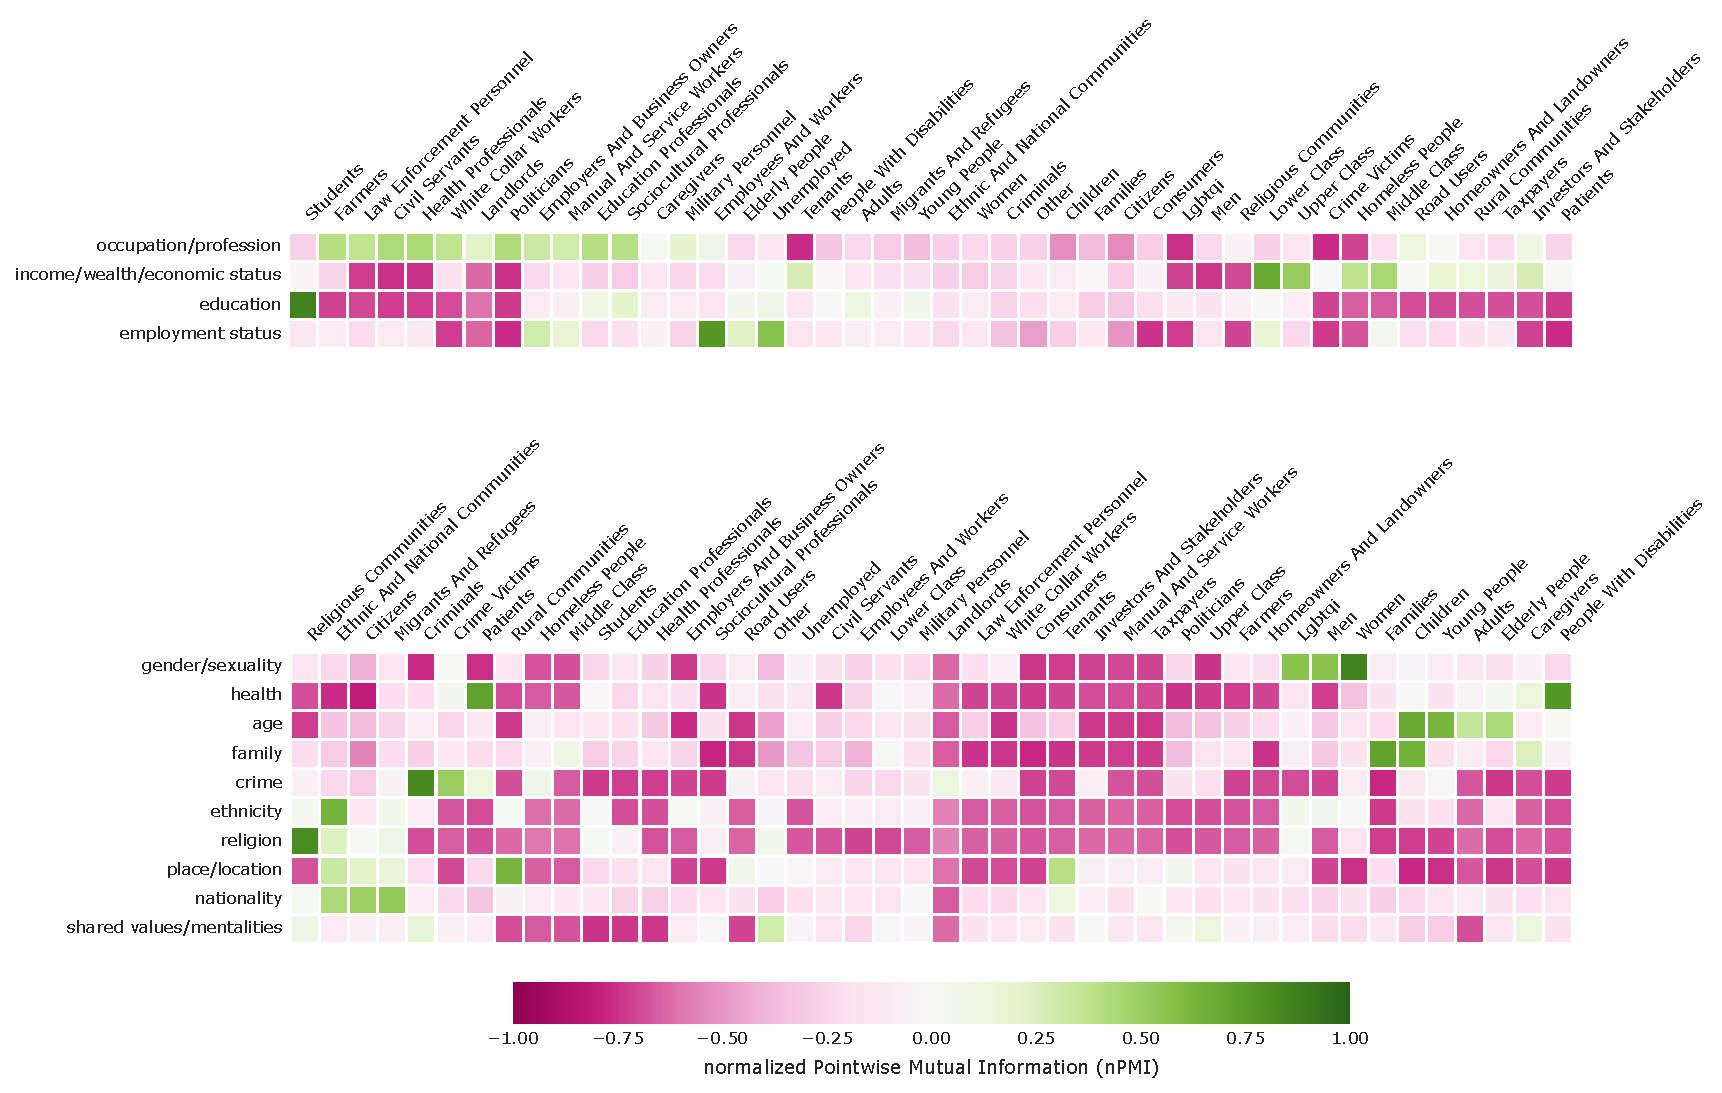
\includegraphics[keepaspectratio,width=\linewidth]{figures/figureC05.pdf}
  \caption{\label{figureC05}\protectPatterns of convergence between group mention classifications of our attribute-centered classifier and Horne et al.'s group category classifier. The figure reports normalized \emph{Pointwise Mutual Information} (nPMI) values that measure the strength of association of label classes on a scale ranging from -1 (systematic disassociation) through 0 (independence) to +1 (perfect co-occurrence).  y-axis labels indicate the attribute category in our scheme; x-axis labels the group categories in Horne et al.'s scheme. Plot panels separated by economic and non-economic attributes. \emph{Note:} heatmap columns sorted (for each attribute dimension) using hierarchical clustering to better reveal conceptual overlap.}
\end{figure}%

Figure~\ref{figureC05} presents the results of this analysis, reporting our attribute categories on the vertical axis and Horne et al.'s group categories along the horizontal axis (sorted to emphasize co-occurrence patterns).
Squares shaded green in Figure~\ref{figureC05} reveal expected convergence patterns, such as the strong co-occurrence tendency of our \emph{occupation/profession} attribute and Horne et al.'s occupation-related categories (e.g., \emph{Civil Servants}, \emph{Farmers}, \emph{Health Professionals}, etc.).
Squares shaded magenta, on the other hand, highlight the attribute categories that are systematically \emph{not} co-occurring with certain group categories in Horne et al.'s scheme.
For example, non-economic attributes like \emph{religion}, \emph{ethnicity}, and \emph{family} show consistent negative associations with occupation- and class-based group categories, because the group mentions sampled from our corpus are typically categorized as either occupation/class-based or non-economic but rarely both at the same time.
Taken together, these positive and negative association patterns reveal systematic similarities in how the two classification schemes partition the social group mention space: attributes that Horne et al.'s classifier treats as separate categories (e.g., occupation versus family status) show mutual exclusivity in their co-occurrence patterns.\footnote{A \(chi^2\)-test computed on the label category co-occurrence count matrix indicates a highly significant overall association between the two classification schemes (\(chi^2\) = 83,259.38, p \textless{} 0.001, Cramér's V = 0.633).}

However, Figure~\ref{figureC05} also shows that our attribute-centered approach groups some of Horne et al.'s more granular categories together (e.g., all occupation-related categories).
Other categories in Horne et al.'s scheme, like \emph{Ethnic And National Communities}, are represented as a mixture of \emph{ethnicity}, \emph{nationality}, \emph{religion}, and/or \emph{place/location} attributes in our scheme.
 
To shed more light on the convergence and divergences between our attribute classification and the group categorization scheme by Horne et al. (2025), we analyze the set of social group mentions labeled as featuring the \emph{occupation/profession} attribute and mentions labeled as featuring the \emph{gender/sexuality} attribute, respectively, in the subset of social group mentions in our machine-labeled corpus originally written in languages in which Horne et al.'s classifier has been evaluated.

This analysis of samples of social group mentions labeled as featuring \emph{occupation/profession}-related and \emph{gender/sexuality}-related attributes, respectively, allows us to assess convergent validity by examining whether the sampled social group mentions are similarly categorized by Horne et al.'s group category classifier.
The dual classification creates overlapping annotations that reveal both areas of agreement (where both schemes identify similar patterns) and divergence (where our attribute-based approach captures distinctions not present in their categorical scheme).
This comparison helps assess to what extent our attribute-centered framework aligns with established categorization but also adds analytical value.
Importantly, we examine these examples not to suggest that our classifiers have a higher accuracy but to illustrate how our attribute-centered approach seems to be better suited to accommodate attribute combinations because it puts all attribute categories on the same analytical level.

\subparagraph{\texorpdfstring{\emph{Occupation/profession}-related social group references}{Occupation/profession-related social group references}}\label{occupationprofession-related-social-group-references}

First, we focus on categories in Horne et al.'s classification scheme that capture references to specific occupational or professional groups.
In total, we identified 14 such categories in their scheme, ranging from \emph{Caregivers} to \emph{White Collar Workers}.\footnote{\emph{Caregivers}, \emph{Civil Servants}, \emph{Education Professionals}, \emph{Employees And Workers}, \emph{Employers And Business Owners}, \emph{Farmers}, \emph{Health Professionals}, \emph{Investors And Stakeholders}, \emph{Law Enforcement Personnel}, \emph{Manual And Service Workers}, \emph{Military Personnel}, \emph{Politicians}, \emph{Sociocultural Professionals}, \emph{White Collar Workers}}

Regarding convergence between their and our annotation scheme, we expect that our focus on occupation/profession-related attributes will lead to a high degree of overlap with mentions categorized into one or several of these categories by Horne et al.' classifiers.
This is confirmed by our analysis, which finds that the share of mentions labeled as expressing an \emph{occupation/profession} attribute by our classifier that are classified into an occupation group category by Horne et al.'s classifier is 84\% -- a high degree of correspondence.

\begin{figure}[!th]

  \centering
  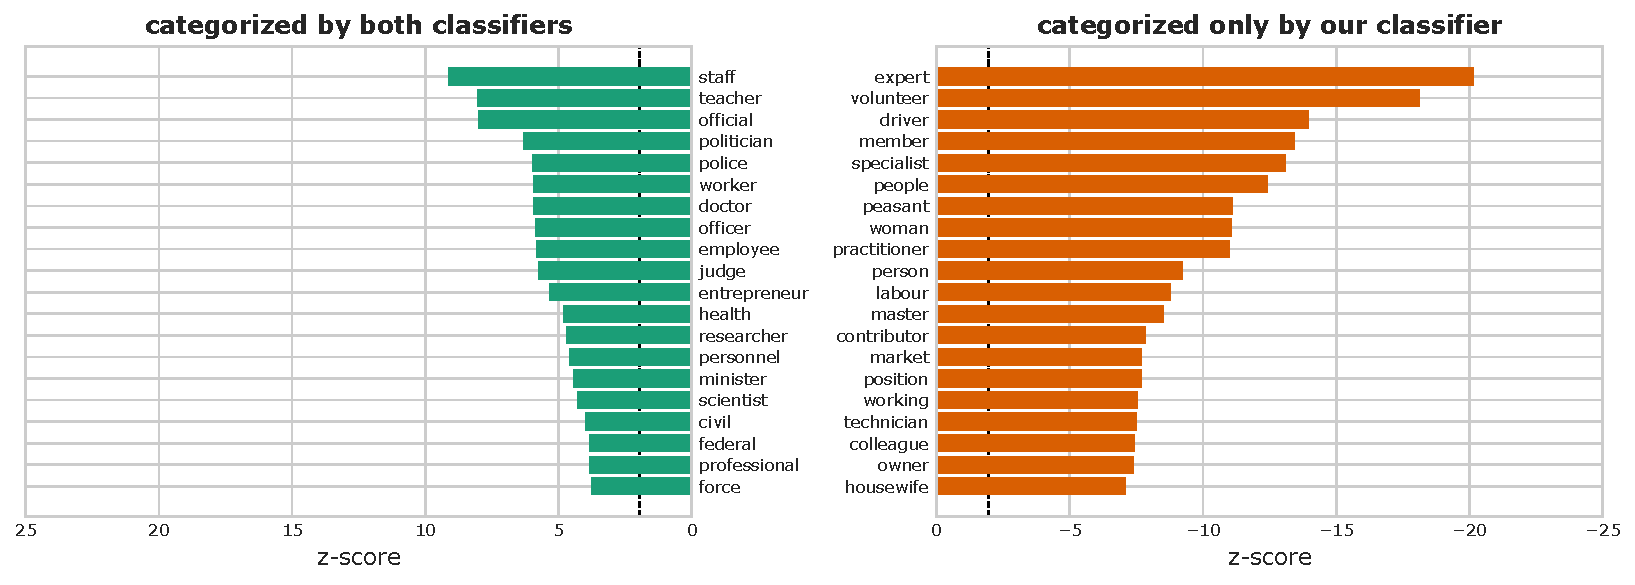
\includegraphics[keepaspectratio,width=\linewidth]{figures/figureC06.pdf}
  \caption{\label{figureC06}\protectMost distinctive words for mentions labeled as featuring occupation/profession as an attribute by our classifier depending on whether Horne et al.'s classifier has classified them into (at least) one of their occupation/profession-related categories (left) or not (right). Values plotted are $z$-scores from ``fighting words'' analysis of occupation/profession mentions. Values above ±1.96 (vertical dashed line) can be considered significantly distinctive.}

\end{figure}%

\begin{table}[!th]
\centering
\caption{Examples of social group mentions labeled as featuring occupation/profession as an attribute by our classifier that were not assigned to any of Horne et al.'s occupation-related group categories by their classifier. Values computed by summing ``fighting words'' scores as weights of mentions' tokens, normalized by number of tokens.}
\label{tableC11}
\begin{tabular}{p{3in} l l}
\toprule
Mention & $z$-score & Horne et al. classification \\
\midrule
International experts & -20.157 &  \\
The volunteers & -18.135 & Other \\
the people smuggler & -12.406 & Criminals \\
-competent people & -12.406 &  \\
environmental experts across Britain & -11.563 & Other \\
experts of interest organisations & -11.526 &  \\
low-skilled women & -11.089 & Women \\
returning volunteers & -9.098 & Other \\
unskilled tax experts who believe to know & -8.603 &  \\
a car and motorcycle driver & -7.419 & Road Users \\
a committee of specialists & -6.954 &  \\
drivers who continue their training in economical and environmentally friendly driving & -6.177 &  \\
human rights representatives in all German embassies & -5.366 & Other \\
legal practitioners & -5.351 &  \\
rail users & -4.652 & Road Users \\
Anyone who collects data and works with it & -4.476 &  \\
concrete and direct owners of what has been & -3.485 & Homeowners And Landowners \\
the respective stakeholder representatives & -3.192 & Other \\
union stakeholders & -2.521 & Other \\
those most directly involved in some of the economic organisations we already have & -2.324 &  \\
\bottomrule
\end{tabular}
\end{table}
%

However, we also expect that due to being more encompassing and abstract than some of Horne et al.'s categories, such as \emph{Civil servants}, \emph{Farmers}, \emph{Health professionals}, etc., our \emph{occupation/profession} attribute will capture a broader set of mentions.
We again assess this question through a ``fighting words'' analysis to identify \(n\)-gram patterns that distinguish the 18\% of social group mentions labeled as featuring the attribute of \emph{occupation/profession} by our classifier that are not classified into any of Horne et al.'s occupation-related categories.
Figure~\ref{figureC06} and Table~\ref{tableC11} show that our \emph{occupation/profession} classifications capture occupational and professional groups not covered by Horne et al.'s schemes, including broad categories like ``experts'' and ``practitioners'' as well as specific categories like ``drivers''.

\subparagraph{\texorpdfstring{\emph{Gender/sexuality}-related social group references}{Gender/sexuality-related social group references}}\label{gendersexuality-related-social-group-references}

Turning to mentions that feature attributes related to gender and/or sexuality, we perform a similar cross-validation exercise by comparing their overlap with classifications into Horne et al.'s group categories \emph{LGBTQI}, \emph{Men}, and \emph{Women}.
Again, we find a high overlap between classifications.
91.9\% of mentions labeled as expressing a \emph{gender/sexuality} attribute by our classifier are classified into (at least) one of Horne et al.'s \emph{LGBTQI}, \emph{Men}, or \emph{Women} group categories by their classifier.

\begin{figure}[!th]

  \centering
  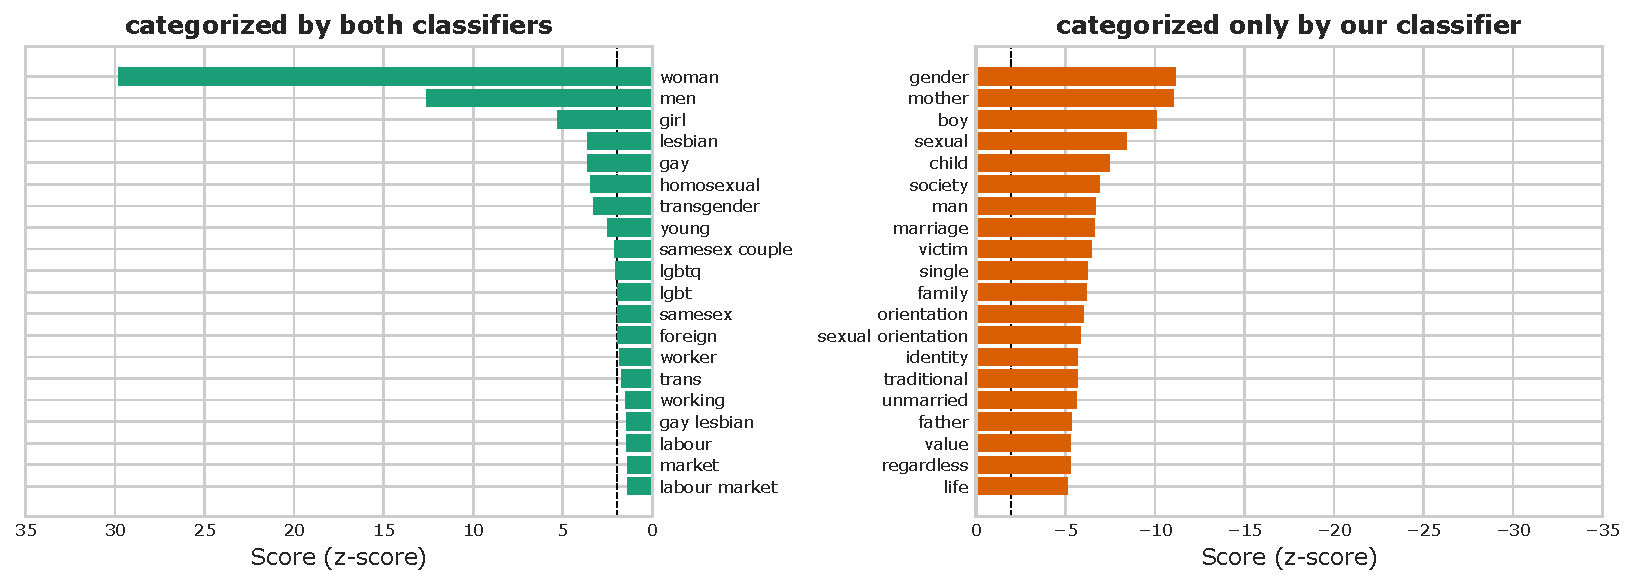
\includegraphics[keepaspectratio,width=\linewidth]{figures/figureC07.pdf}
  \caption{\label{figureC07}\protectTop 20 most distinctive words for gender/sexuality mentions classified by Horne et al. (right) vs. not classified (left).}

\end{figure}%

\begin{table}[!th]
\centering
\caption{Examples of social group mentions labeled as featuring gender/sexuality as an attribute by our classifier that were not assigned to any of Horne et al.'s Men, Women, or LGBTQI categories by their classifier. Values computed by summing ``fighting words'' scores as weights of mentions' tokens, normalized by number of tokens.}
\label{tableC12}
\begin{tabular}{p{3in} l l}
\toprule
Mention & $z$-score & Horne et al. classification \\
\midrule
all genders & -11.141 &  \\
specialized agents on gender issues & -11.141 & Law Enforcement Personnel \\
Familial mothers & -11.036 & Families \\
mothers of 1 or 2 children & -9.258 & Families \\
mothers who have raised at least three children or raised a disabled child & -9.258 & Families \\
a mother and father who & -8.193 & Families \\
a mother who are married & -8.027 & Families \\
the family of father, mother and children & -7.512 & Families \\
people of each gender & -6.715 & Other \\
those who are practically single & -6.250 & Families \\
A society built on solidarity and where we stand up for gender equality and justice & -5.800 & Other \\
everyone, regardless of economics, gender and social status & -5.662 & Other \\
widowed mothers & -5.641 & Families \\
people of all races, religions, sexual orientations, and gender identities & -5.081 &  \\
two cohabitants (married or not & -5.018 & Families \\
People who are not safe in their country on individual grounds (such as sexual orientation, political beliefs or religion & -4.469 & Other \\
mothers and fathers who want to reduce their daily working hours in order to have time for their children & -4.365 & Families \\
couples, whether in marriage & -4.106 & Families \\
well-educated sisters, who have already experienced equality in everyday life & -3.432 & Families \\
fathers who have given up on work after the birth of their children & -3.037 & Families \\
\bottomrule
\end{tabular}
\end{table}
%

However, looking at the remaining mentions that we label as \emph{gender/sexuality}-related but not Horne et al.'s classifier, we again find interesting patterns.
Most common are mentions including the familial role ``mother'' (see Figure~\ref{figureC07}), some of which combine this attribute with qualifiers (see Table~\ref{tableC12}).

\section{Additional results}\label{additional-results}

\subsection{Attribute category focus by party family}\label{attribute-category-focus-by-party-family}


Figure~\ref{figureD01} and Figure~\ref{figureD02} show that the differences between PRR and Green parties' group attribute focus shown in Figure~\ref{figure05} exhibit interesting temporal patterns.
Figure~\ref{figureD01} shows that while their relative emphasis differences are overall very stable across decades, PRR parties' overall stronger focus on the \emph{occupation/profession} attribute is more pronounced in the 1970s than in later decades.
Regarding non-economic attribute prevalence, Figure~\ref{figureD02} shows that Green parties' \emph{age} focus stands out especially in the 2000s and 2010s, whereas their \emph{gender/sexuality} focus has been relatively more pronounced before the 2000s.
PRR parties' group focus, in turn, shows a sharp increase in the prevalence of \emph{family} from 2010s to 2020s.

\begin{figure}[!ht]
  \centering
  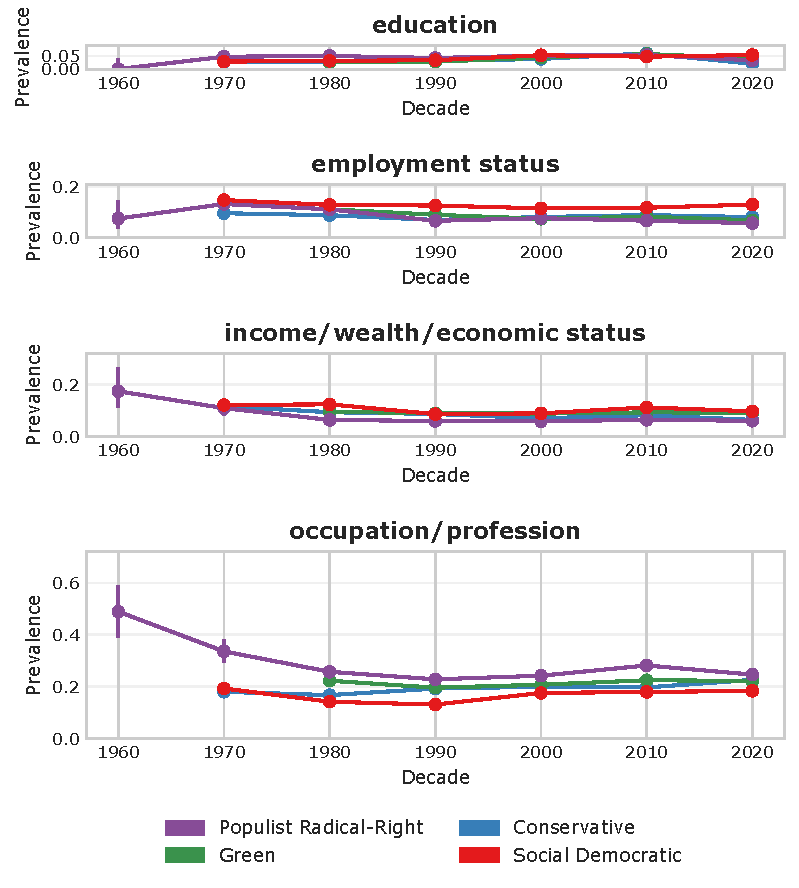
\includegraphics[keepaspectratio,width=0.7\linewidth]{figures/figureD01.pdf}
  \caption{\label{figureD01}\protectTemporal trends in the prevalence of economic attributes in social group mentions by PRR and Green parties across decades. Each panel shows one economic attribute category, with error bars representing 95\% confidence intervals. Lines show the share of mentions containing each attribute over time.}
\end{figure}%

\afterpage{
  \clearpage
  \thispagestyle{empty}
  \begin{figure}[p]
    \centering
    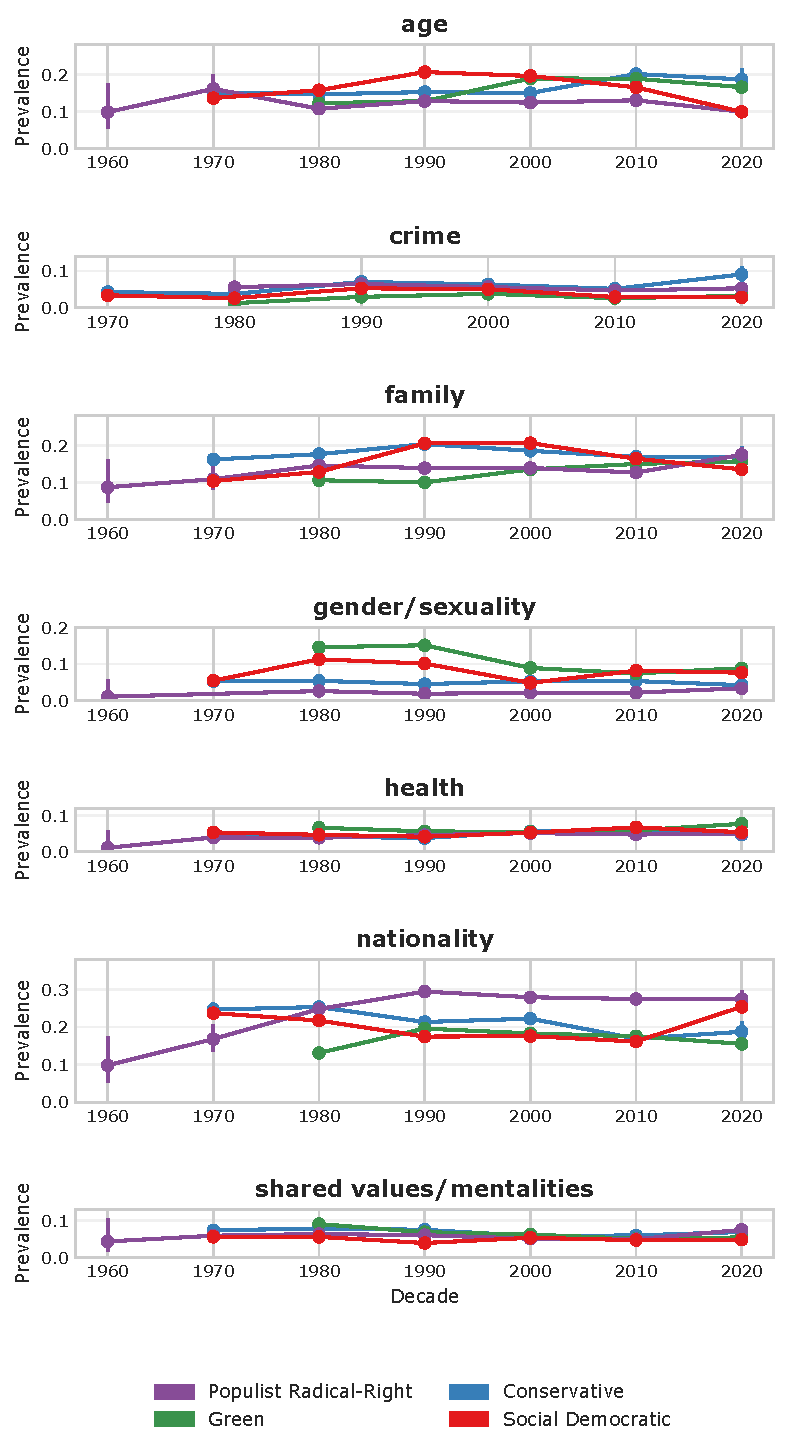
\includegraphics[keepaspectratio,width=0.7\linewidth]{figures/figureD02.pdf}
    \caption{\label{figureD02}\protectTemporal trends in the prevalence of economic attributes in social group mentions by PRR and Green parties across decades. Each panel shows one economic attribute category, with error bars representing 95\% confidence intervals. Lines show the share of mentions containing each attribute over time.}
  \end{figure}%
  \clearpage
}

\subsubsection{Representativeness of our mainstream party selection}\label{sec-apx_case_selection_robustness}

Our case selection strategy aims to cover Green and PRR parties as comprehensively as possible while covering Social Democratic and Conservative parties in four selected countries.
Below, we replicate our analysis of the prevalence of attribute dimensions and categories to assess the representativeness of the cases in the four countries in which we also cover Social Democratic and Conservative parties.

This analysis relies on the \emph{Manifesto Corpus Translations} corpus (Ivanusch and Regel 2024) that records full-text translations for a subset of the manifestos in the Manifesto Corpus.
This data allows us to apply our group mention detection and attribute classifiers also to (quasi-)sentences in cases we have not originally covered in our case selection.

The caveat of this corpus -- and the reason we have not based our raw data collection solely on it -- is that the translations are only available for manifestos for which the Manifesto Corpus records quasi-sentence level annotations.
This is largely only the case for manifestos from elections in the 1990s and later decades -- a much shorter period than we are able to cover through complementary data collection.

As a consequence, only 72 of the 110 mainstream party manifestos covered in our corpus are also covered in the \emph{Manifesto Corpus Translations} corpus (37 from Social Democratic and 35 from Conservative and Christ-Democratic parties).
Yet, the upside of using the \emph{Manifesto Corpus Translations} corpus is that we can cover an additional 492 manifestos (291 Conservative/Christ-Democratic and 201 Social Democratic) in the countries in our case selection.

\afterpage{
  \clearpage
  \thispagestyle{empty}
  \begin{figure}[p]
    \centering
    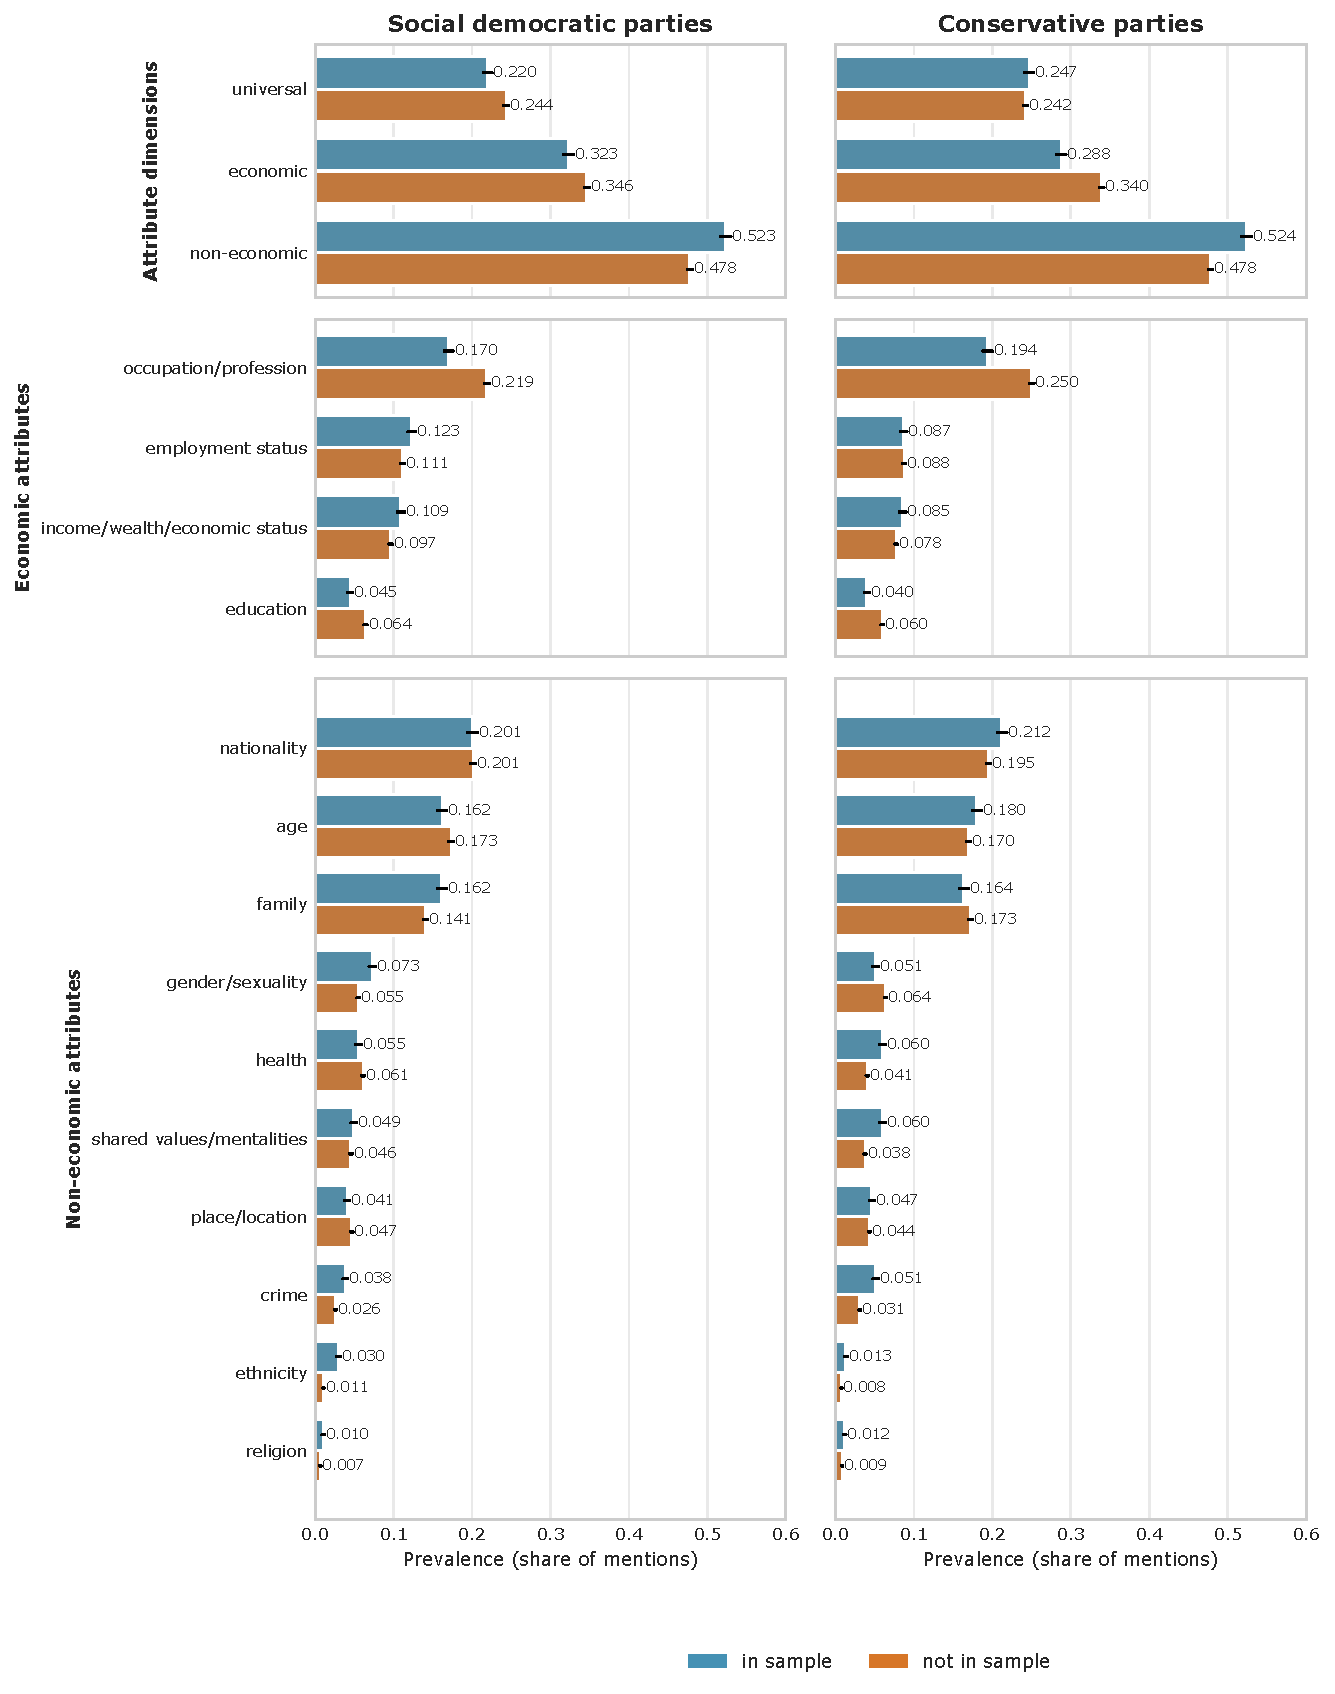
\includegraphics[keepaspectratio,width=\linewidth]{figures/figureD03.pdf}
    \caption{\label{figureD03}\protectPrevalence of attribute dimensions in all mentions and economic and non-economic attributes in non-universal social group mentions in parties' election manifestos by party family. Bars show share of mentions containing each attribute, with 95\% confidence intervals. \emph{Note:} Top panel shows prevalence in all mentions, while middle and bottom panels show prevalence in mentions containing at least one attribute.}
  \end{figure}%
  \clearpage
}

Figure~\ref{figureD03} shows that for most attribute dimensions and categories, the prevalence estimates for parties included and excluded in our case selection are very similar.
However, we observe the following (slight) deviations (compare also to Figure~\ref{figure05}):

\begin{itemize}
\tightlist
\item
  economic dimension: We underestimate Conservative parties' focus on economic attributes.
Adjusting for this makes their emphasis of economic attributes about as high as that of Social Democratic and PRR parties
\item
  non-economic dimension: We slightly overestimate Social Democratic and Conservative parties' focus on non-economic attributes.
Adjusting for this makes their emphasis of non-economic attributes about as high as that of Green and PRR parties.
\item
  \emph{occupation/profession}-related attributes: We slightly underestimate Social Democratic and Conservative parties' focus on occupation/profession.
In pure comparison to Green and PRR parties, this makes these parties (but especially PRR parties) seem slightly more outstanding in this regard than they are in this sample with broader coverage
\end{itemize}

It is worth noting, however, that the differences in prevalence can also be due to differences in the temporal coverage of our case selection and that allowed by relying on the Manifesto Corpus Translation corpus.

\subsection{Conditional probabilities of attribute category co-occurrences}\label{conditional-probabilities-of-attribute-category-co-occurrences}

An alternative approach to quantitatively describing attribute co-occurrence patterns is to compute the conditional probabilities of co-occurrence.
We can compute \(\Pr(\text{attribute B} \mid \text{attribute A})\) for attribute category pairs and compare these values.
Conditional probabilities have the advantage that they are very interpretable, allowing statements like ``When a party uses \emph{economic status} to describe a group, the probability that it also uses \emph{gender/sexuality} in the group mention is 0.12.''
Conditional probabilities thus directly answer substantive questions about co-occurrence patterns.
Further, they do not suffer from base rate sensitivity issues.

The downside is that the measure is asymmetric, requiring careful interpretation.
Further, it does not account for statistical significance of observed differences.
We therefore use it solely for \emph{descriptive} comparison of party families' attribute combination strategies.

\begin{figure}[!th]
  \centering
  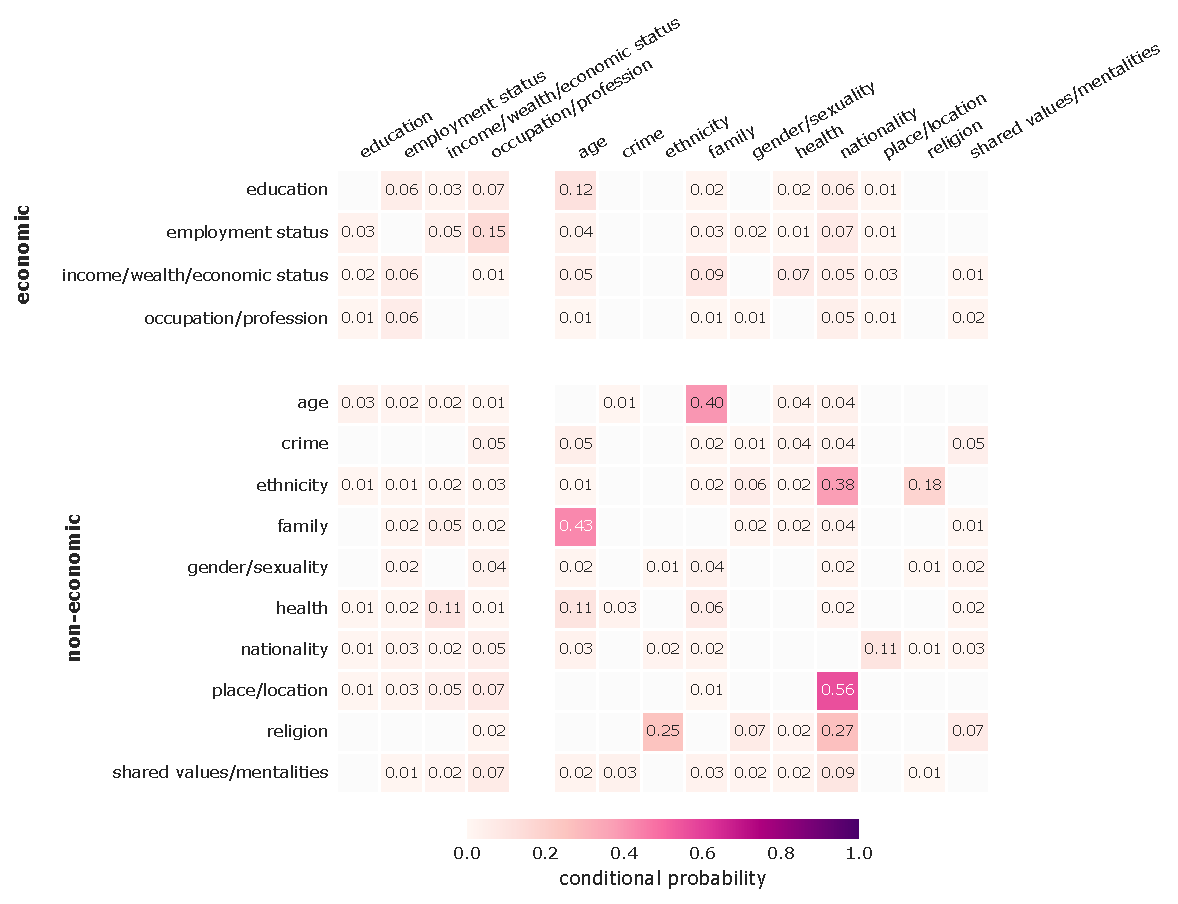
\includegraphics[keepaspectratio,width=\linewidth]{figures/figureD04.pdf}
  \caption{\label{figureD04}\protectConditional probabilities of attribute co-occurrence in social group mentions. Heatmap cells show P(B|A), the probability of mentioning attribute B given that attribute A is mentioned. Rows indicate "attribute A" (the conditioning attribute) and columns indicate "attribute B" (the outcome attribute). \emph{Note:} Values below 0.01 are not displayed.}
\end{figure}%
  

\afterpage{%
  \clearpage%
  \thispagestyle{empty}%
  \begin{landscape}%
  \begin{table}[!th]
\centering
\caption{Top attribute combinations by conditional probability $\Pr(b | a)$, that is, the probability of attribute $b$ being present in a mention given that attribute $a$ is present. Only combinations with $\Pr(b | a) > 0.1$ are included. Example mentions are randomly sampled from mentions that feature both attributes and no other attributes (i.e., mentions that only feature these two attributes).}
\label{tableD01}
\begin{tabular}{p{3cm} L{3cm} r L{2.5cm} L{2.5cm} L{2.5cm} L{2.5cm} L{2.5cm}}
\toprule
attribute a & attribute b & Pr(b | a) & example 1 & example 2 & example 3 & example 4 & example 5 \\
\midrule
place/location & nationality & 0.562 & the population of Africa, including all Arab countries & people in the global South & Foreigners living in Germany & Foreigners residing in Flanders & Nordic citizens who have had a permanent residence in the country for 3 years \\
family & age & 0.429 & children & children & children & children & children \\
religion & nationality & 0.269 & Muslims in France & persecuted minorities in authoritarian states & the second largest religious group in Germany & Islamic faith communities in Germany & most of us \\
religion & ethnicity & 0.255 & a multi-ethnic society & its diverse society & Black and Latino communities & ethnic and cultural minorities & those who attack or derogate any race or creed \\
health & income/wealth/economic status & 0.113 & , who cannot afford the necessary "extras" in medical care from their own pockets & those affected & vulnerable residents & persons with reduced mobility & the affected \\
health & age & 0.107 & healthy and confident young people who have quality medical care & preschool children with special needs & young people with special support needs & the elderly and disabled & elderly people in need of care \\
\bottomrule
\end{tabular}
\end{table}
%
  \end{landscape}%
  %\clearpage%
}%



\end{document}
